%----------------------------------------------------------------------------------------
%	PACKAGES AND OTHER DOCUMENT CONFIGURATIONS
%----------------------------------------------------------------------------------------
\documentclass[
12pt,
english,
singlespacing,
headsepline
]{MastersDoctoralThesis}

\usepackage[utf8]{inputenc}
\usepackage[T1]{fontenc}

\usepackage{fontspec}
\setmainfont{Times New Roman}

\usepackage{caption}
\usepackage{subcaption} 
\usepackage{adjustbox}
\usepackage{tabularx}
\usepackage{rotating}
\usepackage{tikz}

\usepackage{graphicx}
\usepackage[table,xcdraw]{xcolor}

\usepackage[backend=bibtex, sorting = none]{biblatex}
\addbibresource{bibliography.bib}

\usepackage[autostyle=true]{csquotes}
\usepackage{fancyhdr}
\usepackage{tocloft}
\usepackage{titlesec}
\usepackage{float}
\usepackage{placeins}
\let\cleardoublepage=\clearpage

\setlength{\cftbeforechapskip}{10pt}
\setlength{\cftbeforesecskip}{5pt}
\setlength{\cftbeforesubsecskip}{5pt}

\geometry{
	paper=a4paper,
	inner=2.5cm,
	outer=3.5cm,
	bindingoffset=.5cm,
	top=2.5cm,
	bottom=2.5cm,
    right=2.5cm,
}

%----------------------------------------------------------------------------------------
%	THESIS INFORMATION
%----------------------------------------------------------------------------------------

\thesistitle{The impact of computational structural descriptions of PFAS compounds on the performance of classification models estimating their half-lives}
\supervisor{REDACTED_SUPERVISOR}
\author{REDACTED AUTHOR1 NAME, REDACTED AUTHOR 2 NAME}
\keywords{}

\university{\textcolor{blue}{\href{UNI WEBSITE}{REDACTED UNI NAME}}}
\department{\textcolor{blue}{\href{CATHEDRAL WEBSITE}{Wydział Chemii}}}

\AtBeginDocument{
\hypersetup{pdftitle=\ttitle}
\hypersetup{pdfauthor=\authorname}
\hypersetup{pdfkeywords=\keywordnames}
\hypersetup{colorlinks = true, linkcolor = black}
}

\newenvironment{conditions}
  {\par\vspace{\abovedisplayskip}\noindent\begin{tabular}{>{$}l<{$} @{${}={}$} l}}
  {\end{tabular}\par\vspace{\belowdisplayskip}}

\onehalfspacing

\begin{document}

\onehalfspacing
\renewcommand{\chaptername}{Chapter}
\renewcommand{\authorshipname}{Declarations}
\renewcommand{\contentsname}{Table of contents}
\renewcommand{\figurename}{Figure.}
\renewcommand{\listfigurename}{Figure list}
\renewcommand{\listtablename}{Table list}
\newcommand\setrow[1]{\gdef\rowmac{#1}#1\ignorespaces}
\newcommand\clearrow{\global\let\rowmac\relax}
\frontmatter
\setlength{\emergencystretch}{10pt}

\pagestyle{plain}

%----------------------------------------------------------------------------------------
%	TITLE PAGE
%----------------------------------------------------------------------------------------

\begin{titlepage}
\begin{left}

\includegraphics[width=0.5\textwidth]{ug_logo.png} \\[0cm]
\end{left}
\vspace*{0cm}

\begin{center}
{\LARGE\bfseries University of Gdańsk\\[0.5em]
Faculty of Chemistry}\\[1.25cm]

{\bfseries\Large Julia Neumann, Student registration no.: 274301\\}
Field of study: Chemistry 2nd degree\\
Specialisation: Digital Chemistry\\
\\[1cm]
{\bfseries\Large Jakub Rudziński, Student registration no.: 274294\\}
Field of study: Chemistry 2nd degree\\
Specialisation: Digital Chemistry\\

\\[1cm]

{\bfseries\LARGE The impact of computational structural descriptions of PFAS compounds on the performance of classification models estimating their half-lives}\\[0.5cm]

{\Large\textit{\textbf{Wpływ dokładności opisu struktury związków PFAS metodami chemii komputerowej na jakość modeli klasyfikacyjnych stosowanych do szacowania ich okresu półtrwania}}}\\[1cm]

\begin{flushright}
Diploma thesis completed at the\\
Laboratory of Environmental 
Chemoinformatics\\
under the supervision of\\
dr hab. Agnieszka Gajewicz-Skrętna
\end{flushright}
\\
{\textbf{Gdańsk 2025}}

\end{center}
\end{titlepage}

%\cleardoublepage
%\begin{left}
%
\includegraphics[width=0.5\textwidth]{ug_logo.png} \\[0.5cm]
%\end{left}
%\thispagestyle{empty}
%\vspace*{1cm}
%\begin{center}
%\end{center}

\cleardoublepage
\thispagestyle{empty}




%----------------------------------------------------------------------------------------
%	LIST OF CONTENTS/FIGURES/TABLES PAGES
%----------------------------------------------------------------------------------------

\tableofcontents

%----------------------------------------------------------------------------------------
%	THESIS CONTENT - CHAPTERS
%----------------------------------------------------------------------------------------

\mainmatter

\pagestyle{thesis}

% Chapter 0
%\chapter*{}
%\label{Chapter0}

%----------------------------------------------------------------------------------------
\newcommand{\keyword}[1]{\textbf{#1}}
\newcommand{\tabhead}[1]{\textbf{#1}}
\newcommand{\code}[1]{\texttt{#1}}
\newcommand{\file}[1]{\texttt{\bfseries#1}}
\newcommand{\option}[1]{\texttt{\itshape#1}}

%----------------------------------------------------------------------------------------
\clearpage
%\chapter*{Abstract}
\chapter*{\vspace*{-2em} Abstract}
\addcontentsline{toc}{chapter}{Abstract}
\vspace{-1.2cm}
\textbf{The impact of computational structural descriptions of PFAS compounds on the performance of classification models estimating their half-lives}

\vspace{0.2cm}

Per- and polyfluoroalkyl substances (PFAS) are persistent, bioaccumulative chemicals of growing concern due to their resistance to degradation and widespread presence in the environment. This master’s thesis investigates using density functional theory (DFT)-derived molecular descriptors combined with machine learning to predict PFAS persistence in terms of biological half-lives. Our objectives are to evaluate how the choice of quantum chemical method (specifically functional and basis set) influences descriptor reliability, to identify cost-effective computational strategies, and to analyze the impact of individual descriptors on classification performance.

Using three DFT functionals (B3LYP, M06-2X, and ωB97X-D) and three basis sets (6-31G(d,p), 6-31++G(d,p), and cc-pVTZ), we studied nine representative PFAS compounds. Key electronic descriptors, such as the HOMO–LUMO gap, chemical hardness, chemical potential, and electrophilicity, were calculated and shown to be particularly sensitive to method choice.

Three machine learning algorithms—k-nearest neighbors (kNN), decision tree (DT), and extreme gradient boosting (XGBoost)—were trained using descriptor sets from various DFT methods, supplemented with cheminformatics features and two biological descriptors, species and sex. The obtained qualitative structure–property relationship ([Q]SPR) models classified compounds into short-, medium-, or long-half-life categories. The best-performing model, XGBoost with ωB97X-D/cc-pVTZ descriptors, achieved approximately 90\% accuracy, while mid-level methods yielded similar results with significantly lower computational cost.

These results show that DFT-derived descriptors improve PFAS persistence classification and that method selection significantly affects descriptor quality. We propose a hybrid workflow integrating cheminformatics-based screening with targeted DFT descriptor computation as a scalable, efficient approach for analyzing large PFAS libraries. This work contributes to developing in silico tools for regulatory risk assessment and environmental pollutant prioritization.

\vspace{0.1cm}
\textbf{Keywords:} PFAS, persistence, half-life, density functional theory, molecular descriptors, chemoinformatics, [Q]SAR/[Q]SPR, machine learning, classification algorithms

\clearpage
%\chapter*{Streszczenie}
\chapter*{\vspace*{-2em} Streszczenie}
\vspace{-1.2cm}
\addcontentsline{toc}{chapter}{Streszczenie}

\textbf{Wpływ dokładności opisu struktury związków PFAS metodami chemii komputerowej na jakość modeli klasyfikacyjnych stosowanych do szacowania ich okresu półtrwania}

\vspace{0.2cm}

Substancje per- i polifluoroalkilowe (PFAS) to trwałe, bioakumulujące się substancje chemiczne,
które budzą coraz większe obawy ze względu na ich odporność na degradację i powszechną obecność w
środowisku. Niniejsza praca magisterska bada wykorzystanie deskryptorów molekularnych pochodzących z teorii funkcjonału gęstości (DFT) w połączeniu z uczeniem maszynowym w celu przewidywania trwałości PFAS w kategoriach biologicznych okresów półtrwania. Naszymi celami jest ocena, w jaki sposób wybór metody chemii kwantowej
(w szczególności funkcjonału i bazy) wpływa na niezawodność deskryptorów, identyfikacja opłacalnych strategii obliczeniowych i analiza wpływu poszczególnych deskryptorów na
wydajność klasyfikacji.

Używając trzech funkcjonałów DFT (B3LYP, M06-2X i ωB97X-D) i trzech zestawów bazowych (6-
31G(d,p), 6-31++G(d,p) i cc-pVTZ), zbadaliśmy dziewięć reprezentatywnych związków PFAS.
Obliczono kluczowe deskryptory elektroniczne, takie jak luka HOMO–LUMO, twardość chemiczna, potencjał chemiczny i elektrofilowość, i wykazano, że są one szczególnie wrażliwe na wybór metody.

Trzy algorytmy uczenia maszynowego — k najbliższych sąsiadów (kNN), drzewo decyzyjne (DT) i ekstremalne wzmocnienie gradientu (XGBoost) — zostały przeszkolone przy użyciu zestawów deskryptorów z różnych
metod DFT, uzupełnionych o cechy chemiczno-informatyczne i dwa deskryptory biologiczne,
gatunek i płeć. Uzyskane jakościowe modele relacji struktura–właściwość ([Q]SPR)
klasyfikowały związki do kategorii krótkiego, średniego lub długiego okresu półtrwania. Najlepiej działający
model, XGBoost z deskryptorami ωB97X-D/cc-pVTZ, osiągnął około 90\% dokładności, podczas gdy metody średniego poziomu dały podobne wyniki przy znacznie niższym
kosztach obliczeniowych.

Wyniki te pokazują, że deskryptory pochodzące z DFT poprawiają klasyfikację trwałości PFAS
a wybór metody obliczeń znacząco wpływa na jakość używanych deskryptorów. Proponujemy hybrydowy przepływ pracy integrujący przesiewanie oparte na chemioinformatyce z ukierunkowanymi obliczeniami deskryptora DFT
jako skalowalne, wydajne podejście do analizy dużych bibliotek PFAS. Niniejsza praca przyczynia się do
rozwoju narzędzi in silico do oceny ryzyka regulacyjnego i ustalania priorytetów zanieczyszczeń środowiska.

\vspace{0.1cm}

\textbf{Słowa kluczowe:} PFAS, trwałość, okres półtrwania, teoria funkcjonału gęstości, deskryptory molekularne, chemoinformatyka, [Q]SAR/[Q]SPR, uczenie maszynowe, algorytmy klasyfikacyjne

% Chapter 1
\chapter{Introduction}
\label{Chapter1}

%----------------------------------------------------------------------------------------
\newcommand{\keyword}[1]{\textbf{#1}}
\newcommand{\tabhead}[1]{\textbf{#1}}
\newcommand{\code}[1]{\texttt{#1}}
\newcommand{\file}[1]{\texttt{\bfseries#1}}
\newcommand{\option}[1]{\texttt{\itshape#1}}

%----------------------------------------------------------------------------------------
\vspace{-1cm}
\section{Background and motivation} \label{sec:background_motivation}


The extensive use of PFAS in various industries and consumer products has led to their widespread presence in the environment. PFAS have been detected in various environmental media, including water, soil, and air, as well as in the tissues of wildlife and humans. Due to their chemical stability and resistance to natural degradation processes, PFAS can persist in the environment for decades, posing long-term exposure risks. Their persistence, combined with their ability to bioaccumulate in living organisms, raises serious concerns regarding human health and environmental sustainability~\cite{PFAS_in_animals_humans, PFAS_livestock, PFAS_environ_impacts_health, PFAS_in_water, PFAS_in_drinking_water}.

There is growing evidence that exposure to PFAS substances is associated with a range of adverse health effects. Epidemiological studies have linked PFAS exposure to an increased risk of certain cancers, liver damage, immune systems suppression, thyroid dysfunction, and developmental issues in children~\cite{PFAS_cancers_1, PFAS_cancers_2, PFAS_fatty_liver_USA, PFAS_immune_suppression, PFAS_developmental_issues}.These health concerns are particularly alarming given the widespread presence of PFAS. Studies indicating that nearly all individuals in industrialized nations have detectable levels of these substances in their blood~\cite{PFAS_Italy}. The potential for chronic health effects, combined with the persistence and bioaccumulative nature of PFAS, has heightened intensified public and scientific interest in understanding and mitigating

The regulatory landscape for PFAS is evolving rapidly as governments and environmental agencies respond to the growing body of evidence regarding their environmental and health impacts. In the United States, for example, the Environmental Protection Agency (EPA) has begun establishing health advisories and regulatory limits for certain PFAS compounds in drinking water. Similar efforts are underway in other countries, particularly within the European Union, where restrictions on specific PFAS compounds are being implemented. However, the vast number of PFAS substances, combined with limited toxicological data for many of them, presents significant challenges for regulatory authorities. 

%----------------------------------------------------------------------------------------
\section{Per- and polyfluoroalkyl substances} \label{sec:pfas_intro}

PFAS substances are a group of organic compounds characterized by carbon chains bonded to fluorine atoms. Figure \ref{structure_chapter_2} provides the names, abbreviations, and 2D structures of the more commonly studied PFAS. According to the Organization for Economic Co-operation and Development (OECD)’s latest definition, PFAS are fluorinated substances that contain at least one fully fluorinated methyl or methylene carbon atom ~\cite{2}. PFAS can be classified as short-chain (≤ seven carbon atoms) or long-chain (≥ eight carbon atoms) compounds. Long-chain PFAS are often referred to as “legacy” compounds due to their extensive history of study. The most thoroughly researched long-chain PFAS are perfluorooctane sulfonate (PFOS) and perfluorooctanoic acid (PFOA). Production of these compounds was discontinued in several countries (e.g., the United States in the 2000s) due to their adverse health effects~\cite{2,3}.

The chemical structure of PFAS, particularly its carbon–fluorine (C–F) bonds, includes some of the strongest bonds in organic chemistry. This exceptional bond strength contributes to PFAS’s high resistance to chemical, thermal, and biological degradation. This allows PFAS to persist in the environment and in the human body, where they are difficult to eliminate. PFAS are non-flammable, non-corrosive, and resistant to combustion, degradation, and most chemical reactions. Furthermore, PFAS molecules typically possess both hydrophobic and hydrophilic ends, giving them unique surfactant properties. Their long biological half-lives result in bioaccumulation over time, further complicating efforts to mitigate their impact on human health and the environment. While the production of certain PFAS, such as PFOA and PFOS, was halted in countries like the United States due to their toxicity concerns, these substances still pose significant environmental and health risks~\cite{PFOA_PFOS_risk}.

\begin{figure}[H]
\centering
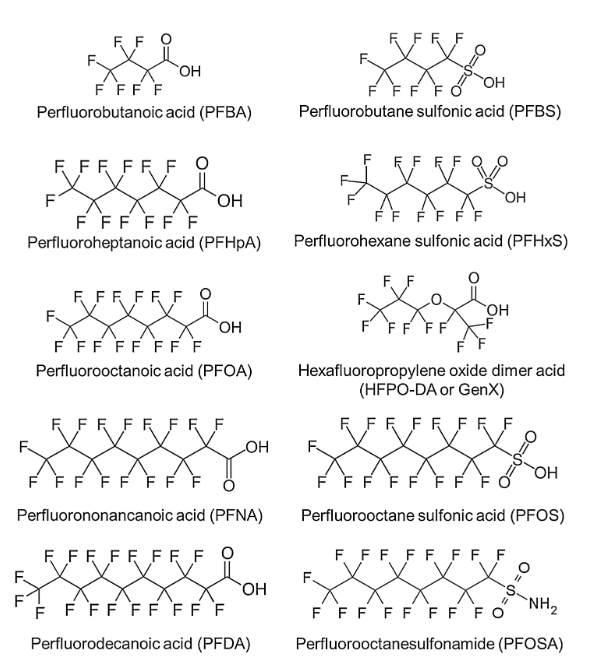
\includegraphics[width=\textwidth,height=\textheight,keepaspectratio]{Figures/structure_chapter_2.png}
\caption{Two-dimensional (2D) chemical structures of selected PFAS and related compounds \cite{structures_graphic}}
\label{structure_chapter_2}
\FloatBarrier
\end{figure}

%----------------------------------------------------------------------------------------
\clearpage
\subsection{Uses and potential risks} \label{sec:uses_risks}

PFAS substances are a group of synthetic compounds widely used in industrial processes due to their resistance to degradation, surfactant properties, and thermal and flame resistance. Their water- and grease-repellent properties make them ideal for food packaging, non-stick cookware, and waterproof textiles. Beyond these applications, PFAS are also found in paints, adhesives, electrical wire insulation, detergents, fire-resistant materials, carpets, and even cosmetics~\cite{3,4}.

One of the most concerning effects of PFAS compounds exposure is their potential impact on thyroid health. Thyroid hormones play a key role in regulating metabolism, and proper thyroid function is associated with cardiovascular health, fertility, and fetal neurodevelopment. Studies have suggested that PFAS may disrupt thyroid hormone regulation, which could potentially affect pregnancy outcomes and the development of fetuses and young children ~\cite{3}.

%----------------------------------------------------------------------------------------
\subsection{Environmental and health concerns} \label{sec:env_health_concerns}

The widespread use of PFAS in various industries, coupled with the chemicals’ stability, has led to significant environmental contamination. PFAS compounds have been detected in surface water, groundwater, soil, and air. Their solubility in water and resistance to degradation allow them to travel long distances from their original source(s), contributing to their global distribution in the environment~\cite{Sweden_distribution}.

Recent epidemiological studies have linked exposure to certain PFAS compounds with adverse health effects. These risks are further compounded by PFAS’s ability to accumulate in the human body over time, particularly in the blood, liver, and kidneys, due to their long biological half-lives. Consequently, even low-level, long-term exposure to PFAS can lead to serious health consequences. Many legacy PFAS, such as PFOA and PFOS, have accumu- lated in the environment, as well as in animals and humans. Mixtures of legacy and newer PFAS continue to be detected in the environment, including in global food and water supplies. The biological half-lives of legacy PFAS in human serum are approximately four years for PFOA, five years for PFOS, and eight and a half years for PFHxS. The biological half-lives of newer PFAS compounds are less well understood, though available studies suggest that they are excreted at significantly faster rates~\cite{4}.

Full defluorination (DeF) or mineralization of PFAS is necessary to eliminate fluoride contamination completely. However, current technologies can only partially defluorinate a limited range of PFAS compounds. In 2023, the U.S. EPA established new drinking water standards for perfluorooctanesulfonic acid (PFOS) and perfluorooctanoic acid (PFOA) at 4.0 parts per trillion (ppt). Achieving this near-zero threshold will require technological innovations that enable the complete defluorination of parent PFAS compounds, rather than merely degrading them. DeF specifically refers to the percentage of fluoride ions released from PFAS molecules. Full DeF is critical because partial defluorination can lead to the formation of  potentially more toxic and persistent short-chain byproducts that are more likely to bioaccumulate in animals and humans~\cite{6}.

%----------------------------------------------------------------------------------------
\subsection{Regulatory challenges and research directions} \label{sec:reg_challenges}

Because of the persistence and toxicity of PFAS, regulatory agencies worldwide have started to implement guidelines and regulations that limit human and environmental exposure. For example, the U.S. EPA has issued health advisories for PFOA and PFOS in drinking water. Although these advisories are not legally enforceable, they are currently under review for potential revision. Similarly, several European Union countries have restricted the use of certain PFAS in consumer products and industrial applications. Despite these efforts, the vast number of PFAS compounds, combined with the lack of comprehensive toxicological data for many of them, continue to pose significant challenges for regulatorss~\cite{PFAS_regulators, PFAS_regulators_2, PFAS_regulators_3}.

Ongoing research is focused on developing more effective methods for detecting and quantifying PFAS in environmental samples and exploring potential remediation strategies. Analytical techniques such as liquid chromatography–mass spectrometry (LC–MS/MS) have become the gold standard for PFAS detection due to their high sensitivity and specificity~\cite{PFAS_detection_1, PFAS_detection_2, PFAS_detection_3, PFAS_detection_4}. Nevertheless, detecting PFAS at environmentally relevant concentrations remains challenging, particularly for emerging PFAS compounds that are not well characterized. 

In terms of remediation, conventional water treatment technologies, such as activated carbon filtration and ion exchange, have been somewhat effective at removing PFAS from contaminated water sources. However, these methods often lack the capacity to address the full spectrum of PFAS compounds present in the environment. Consequently, advanced treatment methods, including high-pressure membrane filtration, advanced oxidation processes, and electrochemical degradation, are being investigated as potential solutions to this complex issue~\cite{PFAS_membrane_filtration, PFAS_oxidation_1, PFAS_oxidation_2}.

% ----------------------------------------
% ----------------------------------------
% ----------------------------------------
\clearpage
\subsection{Methods for determining biological and physicochemical \\properties}

Chemical safety evaluations rely on an understanding of key properties, such as half-life, protein binding, solubility, and membrane permeability. These parameters have traditionally been assessed through \textit{in vivo} studies (i.e., animal testing) or \textit{in vitro} assays (e.g., cell cultures).). In recent years, in silico techniques, particularly qualitative and quantitative structure–activity/property relationships, have gained importance. These techniques offer faster, more ethical and more cost-effective alternatives to laboratory testing. They also enable preliminary hazard screening in scenarios with limited data \cite{Gkika2023, Cherkasov2014}.

\subsection{QSAR/QSPR models for PFAS}

Recent technological advancements, particularly in computing, have led to a steady increase in the use of computer-based approaches, commonly referred to as \textit{in silico} methods, in chemical hazard assessment. Two major categories of \textit{in silico} approaches can be distinguished: (1) qualitative structure-activity/property relationship methods (SAR/SPR also known as [Q]SAR/[Q]SPR) and (2) quantitative structure-activity/property relationship methods (QSAR/QSPR). Both types of methods aim to establish a link between the structural features of a group of chemical compounds and their biological activity (e.g., acute toxicity to \textit{Daphnia magna}) or physicochemical property (e.g., water solubility), through the development of appropriate mathematical models. The primary difference between these two approaches is the type of output they generate. [Q]SAR/[Q]SPR models produce categorical (i.e., discrete) outcomes, whereas QSAR/QSPR models yield numerical (i.e., continuous) predictions. Qualitative methods are generally preferred in the early stages of analysis because they enable the rapid classification of chemical compounds into distinct classes. For example, they can distinguish between biologically active and inactive compounds. This classification typically involves assigning labels such as “toxic” or “non-toxic.”\cite{NevesB}\cite{TsuiM}

The [Q]SAR/[Q]SPR methodology, schematically presented in Figure \ref{fig:SAR_modeling_flowchart}, consists of six main stages, which are briefly described below. 

\begin{figure}[H]
    \centering
    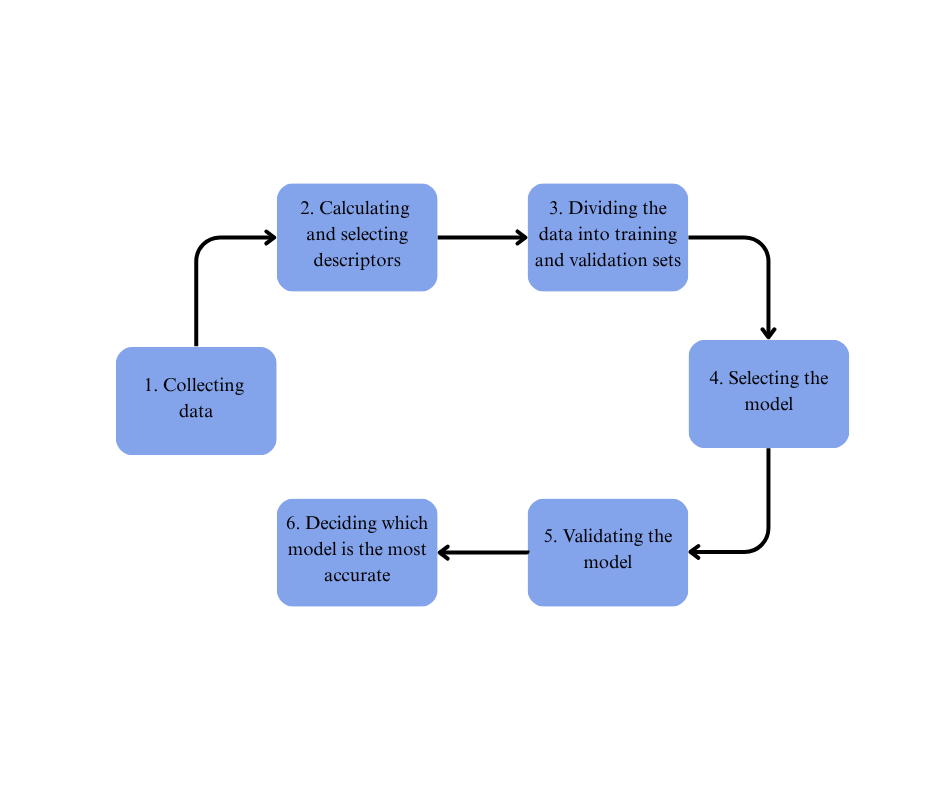
\includegraphics[width=\textwidth,height=\textheight,keepaspectratio]{Figures/SAR.png}
    \caption{[Q]SAR modeling flowchart (own work)}
    \label{fig:SAR_modeling_flowchart}
\end{figure}

The first step in the [Q]SAR/[Q]SPR modeling process is collecting data from experiments, literature, or relevant databases. Next, molecular descriptors are calculated. These descriptors play an important role in [Q]SAR/[Q]SPR modeling because they provide a mathematical representation of the various structural and physicochemical properties of molecules. Depending on how they are obtained, descriptors fall into two categories: (1) experimental, which are determined through laboratory measurements (e.g., water solubility), and (2) theoretical, which are calculated based on chemical composition, structural topology (i.e., the arrangement of atoms in a molecule), or derived from quantum-mechanical calculations based on the 3D molecular structure (e.g., polarizability). A well-chosen descriptor exhibits continuous variability and, most importantly, captures subtle changes in molecular structure \cite{MauriA}. The set of descriptors selected for developing a [Q]SAR/[Q]SPR model should facilitate mechanistic interpretation by linking structural variations to observed changes in biological activity. In other words, the descriptors should provide insight into the underlying mechanism of action, such as the toxic effect of a chemical compound within a biological system.


The third step in the [Q]SAR/[Q]SPR modeling process is to split the collected dataset into two subsets:

\begin{enumerate}
    \item \textbf{The training set}, which is used to build the model. This involves defining logical rules or decision boundaries to classify objects (i.e., compounds) into categories (i.e., two or more classes), in the case of qualitative models;
    \item \textbf{The test set} (also known as validation set), which is used to evaluate the model’s predictive accuracy for compounds not included in the training phase.
\end{enumerate}

The fourth step is selecting an appropriate machine learning (ML) algorithm. This is a crucial step because the modeling technique must align with the nature and complexity of the dataset to capture meaningful relationships. Using an inappropriate ML method can significantly reduce predictive accuracy and increase misclassification rates. Another challenge is the wide array of available modeling techniques, each of which requires tuning specific parameters.

Before a developed [Q]SAR/[Q]SPR model can be applied in practice, it must undergo rigorous validation. This step is essential for assessing the model’s reliability in predicting biological responses or physicochemical properties, for compounds not involved in model development. \cite{NevesB}\cite{Jaganathan}\cite{Polishchuk}

Relatively few [Q]SAR/[Q]SPR models focus specifically on PFAS, primarily due to the limited availability of high-quality experimental data. Existing models often rely on simple one- or two-dimensional (1D or 2D) descriptors, such as molecular weight or n-octanol-water partition coefficient (logP), and tend to overlook more detailed electronic structure descriptors, such as the energy difference between the highest occupied molecular orbital (HOMO) and lowest-unoccupied molecular orbital (LUMO) (HOMO–LUMO gap) or chemical potential \cite{BlakeFenton2020, Gkika2023}. This underscores the necessity of incorporating more sophisticated descriptors to more accurately capture the factors influencing PFAS persistence and toxicokinetics. However, it should be noted that quantum-chemical modeling of PFAS poses challenges, especially when selecting the optimal combination of functionals, basis sets, and polarization and/or diffuse functions. The wide variety of these parameters makes determining the most suitable setup for accurately modeling this unique class of compounds difficult.

 
Therefore, selecting the most appropriate levels of theory adds complexity to geometry optimization, descriptor calculation, and, ultimately, [Q]SAR/[Q]SPR model development. Options include various functionals (e.g., \texttt{B3LYP}, \texttt{M06‑2X}, \texttt{$\omega$B97X-D)}, basis sets (e.g., \texttt{6‑31G}, \texttt{6‑31++G}, \texttt{cc-pVTZ}), and descriptor types (e.g., electronic, geometric, and thermodynamic). Each combination involves trade-offs between computational cost and the accuracy of the resulting descriptors. An optimal workflow should balance model performance and computational feasibility, especially for large-scale screening applications \cite{Gkika2023, Cherkasov2014}.

% ----------------------------------------
% ----------------------------------------
% ----------------------------------------
\chapter{Research hypothesis and objectives}

Given the limitations of existing in silico models, which often rely on simple 1D or 2D descriptors and fail to capture electronic structure, this section outlines the key research questions and hypotheses that guide this master’s thesis.

This thesis primary aims to investigate whether descriptors derived from DFT can improve the prediction of PFAS half-life categories when combined with molecular descriptors generated using RDKit \cite{rdkit} and Open Babel \cite{openbabel}. To explore this, we pose the following three specific research questions:

\begin{enumerate}
  \item Does combining DFT-derived descriptors (i.e., electronic, geometric, and thermodynamic) with RDKit/Open Babel descriptors improve the accuracy with which PFAS are classified into half-life categories compared to models that do not incorporate descriptors based on optimized 3D structure?
  
  \item How does the choice of DFT functional (\texttt{B3LYP}, \texttt{M06‑2X}, \texttt{\(\omega\)B97X‑D}) and basis set (\texttt{6-31G(d,p)}, \texttt{6-31++G(d,p)}, \texttt{cc-pVTZ}) ) influence the robustness of the descriptors and the overall performance of the model, while considering computational time?
  
  \item Is it possible to identify an optimal combination of ML method and descriptor set that balances predictive accuracy with computational efficiency?
\end{enumerate}

Based on these questions, we formulated the following research hypotheses:

\begin{itemize}
  \item H1: Classification models incorporating DFT-derived descriptors will outperform —or at least match—the predictive accuracy of models using only 1D and 2D descriptors, potentially with lower model complexity.
  
  \item H2: The quality of the [Q]SPR models varies depending on the chosen DFT method, however, more computationally expensive methods do not necessarily yield better predictive performance.
  
  \item H3: A combination of DFT method and descriptor set exists that offers high classification performance at a significantly reduced computational cost compared to high-level DFT calculations.
  
  \item H4: The choice of ML algorithm (e.g., k-NN, DT, XGB) significantly impacts both classification performance and model interpretability.
\end{itemize}

To test these hypotheses, the following objectives have been defined:

\begin{enumerate}
  \item Perform DFT optimizations of PFAS structures using the selected functionals and basis sets, and record the computational time required for each.
  
  \item Generate electronic, geometric and thermodynamic descriptors from the optimized molecular geometries.
  
  \item Integrate the DFT-derived descriptors with the original data derived from \cite{dataset_source} , including PFAS half-lives and biological descriptors.
  
  \item Perform feature selection and develop classification models to classify PFAS based on toxicokinetic half-life.
  
  \item Evaluate model performances across different combinations of DFT-derived descriptor sets and ML algorithms to identify the optimal trade-off between accuracy and computational cost.
\end{enumerate}

Through this research workflow, we aim to improve our understanding of how molecular structure, particularly electronic properties, affects PFAS environmental persistence. Additionally, the master’s thesis seeks to deliver a scalable, practical computational workflow for predicting the environmental and human health risk of legacy and emerging PFAS compounds.

 
% Chapter 3

\chapter{Methodology}

\label{Chapter3} 

%----------------------------------------------------------------------------------------

\newcommand{\keyword}[1]{\textbf{#1}}
\newcommand{\tabhead}[1]{\textbf{#1}}
\newcommand{\code}[1]{\texttt{#1}}
\newcommand{\file}[1]{\texttt{\bfseries#1}}
\newcommand{\option}[1]{\texttt{\itshape#1}}

%----------------------------------------------------------------------------------------
\section{DFT calculations}

\subsection{History of density functional theory}

Density functional theory (DFT) is one of the most widely used methods in computational chemistry and materials science. It allows the efficient calculation of electronic structures for molecules and materials. Although DFT's conceptual foundation originated in quantum mechanics, it was formally established in the mid-20th century~\cite{DFT_Origins}.

In 1964, Hohenberg and Kohn demonstrated that the ground-state properties of a many- electron system depend entirely on its electron density, rather than on the complex many-body wavefunction \cite{Hohen_Kohn}. This significantly simplified the problem because electron density depends on only three spatial coordinates.

The following year, Kohn and Sham introduced the Kohn-Sham (KS) equations \cite{Kohn_KS_equations}, reformulating the many-electron problem as a system of non-interacting particles. Electron-electron interactions are incorporated through an exchange-correlation functional. Since the exact form of this functional remains unknown, various approximations have been developed over time. The first widely used functional was the Local Density Approximation (LDA), followed by more accurate methods, such as the Generalized Gradient Approximation (GGA) and hybrid functionals that incorporate Hartree-Fock exchange.

Despite its success, DFT still faces notable limitations. Accurately describing strongly correlated materials, van der Waals interactions, and excited states remains challenging. Standard DFT functionals often have difficulty with systems in which electron correlation plays a significant role, such as transition metal oxides \cite{DFT_strongly_correlated}. Additionally, conventional DFT approaches may inadequately capture dispersion forces, leading to inaccuracies in systems dominated by van der Waals interactions \cite{DFT_vdw_limitations}. Excited-state properties also pose difficulties, as time-dependent DFT (TDDFT) may fail to accurately describe certain excitation phenomena \cite{TDDFT_challenges}.

To address these challenges, ongoing research focuses on improving exchange-correlation functionals and integrating DFT with other computational methods. Researchers are actively pursuing strategies such as combining DFT with many-body perturbation theory (MBPT) and enhancing TDDFT techniques to overcome current limitations and expand the applicability of DFT to a broader range of complex systems \cite{DFT_MBPT_TDDFT}.


\subsection{Basis sets in quantum chemistry}

In this section, we provide a brief overview of the basis sets and functionals employed in this master's project.


Basis sets are fundamental to quantum chemical calculations, because they provide the mathematical functions used to approximate electronic wavefunctions. Since obtaining  exact solution of the Schrödinger equation for many-electron systems is generally infeasible, basis sets enable molecular orbitals to be expressed as linear combinations of predefined functions. This balances computational cost and accuracy. These functions, which are typically centered on atomic nuclei, are designed to capture the spatial and energetic behavior of electrons. The choice of basis set significantly impacts the accuracy of computed properties, such as total energies, dipole moments, and vibrational frequencies, as well as the necessary computational resources.

Different basis sets offer various trade-offs. Minimal basis sets (e.g., STO-3G) are computationally efficient, but they lack flexibility. Split-valence basis sets (e.g., 6-31G and 6-311G) improve accuracy by using multiple functions to describe valence electrons. Polarization functions (denoted by * or **) introduce higher angular momentum components, thereby enhancing the description of bonding and polarization effects. Diffuse functions (indicated by + or ++) expand the spatial extent of basis functions. This expansion is important for accurately describing anions and weakly bound species.

Dunning’s correlation-consistent basis sets (i.e., cc-pVXZ, where X = D, T, Q, etc.) are widely used in correlated wavefunction methods and high-precision DFT calculations because they offer systematic convergence and high accuracy. Augmented variants (aug-cc-pVXZ) include diffuse functions to more accurately capture weak intermolecular interactions. Effective core potentials (ECPs) replace core electrons with pseudopotentials, which significantly reduces the computational demands for heavier elements. 

Selecting a basis set requires balancing accuracy with computational efficiency depending on the system under investigation. Larger basis sets provide greater precision, but at the cost of increased computational time and resources. To improve accuracy further, basis set extrapolation and composite methods are often used to estimate complete-basis-set (CBS) limits.

\subsubsection{Polarizability and the role of diffuse functions in DFT}

Polarizability is a measure of  how an electron cloud deforms in response to an external electric field. It plays a critical role in understanding intermolecular interactions, dielectric properties, and molecular response functions. Accurately calculating polarizability calculations within DFT require precisely representing the electron density, particularly for systems with weakly bound or delocalized electrons. Diffuse functions extend the spatial reach of the basis functions, making them essential for achieving this level of accuracy. 

Diffuse functions denoted by ”+” or ”++” (e.g., 6-31+G), add low-exponent Gaussian functions that allow molecular orbitals to extend further into space. These functions are particularly important for describing anions, excited states, and systems with significant electron delocalization. Including diffuse functions improves the accuracy of computed dipole moments, polarizabilities, and dispersion coefficients. DFT methods that incorporate long-range corrections or dispersion terms, such as LC-DFT, DFT-D, ωB97X-D, and B3LYP-D3, benefit greatly from diffuse-augmented basis sets, as they address the limitations of standard functionals when modeling van der Waals interactions and extended charge distributions. 

For complex molecules, such as fluorinated compounds and highly electronegative species, basis sets with diffuse functions (e.g., aug-cc-pVTZ) are essential for reliably calculating electronic properties. Combining diffuse-augmented basis sets with advanced functionals (e.g., ωB97X-V, M06-2X) enables for the accurate calculating of static and dynamic polarizabilities, solvent effects, molecular interactions, and electrostatic potentials. This makes the approach indispensable in modern computational chemistry.

\subsubsection{The 6-31G(d,p) and 6-31++G(d,p) basis sets}
 
The 6-31G(d,p) and 6-31++G(d,p) basis sets are both part of the Pople split-valence family. They offer an effective balance between computational efficiency and accuracy, making them well-suitable for DFT studies on medium-to-large molecular systems. These basis sets are used in this master’s thesis due to their proven performance in geometry optimization and electronic property calculations. 

The 6-31G split-valence scheme uses six Gaussian primitives for core orbitals and provides flexible valence descriptions with three and one Gaussian functions, respectively. The (d,p) extension introduces polarization functions—d-type functions for non-hydrogen atoms and p-type for hydrogen atoms— thereby enhancing the description of molecular distortions, bonding characteristics, and vibrational properties. 

The ++ augmentation adds diffuse functions: the first + applies to heavy atoms and the second + to hydrogen atoms. These diffuse functions consist of low-exponent Gaussian functions that improve the representation of weakly bound electrons, long-range interactions, and extended charge distributions. These features are essential for accurately modeling anions, Rydberg states, and systems with significant electron delocalization. 

The 6-31G(d,p) basis set is more effective for neutral molecules with localized electron density, as diffuse functions are unnecessary in these cases. It offers computational efficiency without sacrificing accuracy for tasks such as geometry optimization and thermochemical prediction. However, the omission of diffuse functions limits its applicability to anions, charge-transfer complexes, and systems where accurate long-range electrostatics are critical. 

The 6-31++G(d,p) basis set overcomes the limitations of previous models by incorporating diffuse functions. This improves the accuracy of systems involving anions, dipole moments, polarizabilities, van der Waals interactions, and charge-transfer processes. It is particularly beneficial when used with dispersion- corrected functionals, such as DFT-D3, DFT-D4, as it provides a more comprehensive description of long-range correlation effects. However, including diffuse functions increases the computational cost and may introduce numerical instabilities, such as linear dependence, in large systems with weakly interacting fragments. Therefore, the selection of either the 6-31G(d,p) or the 6-31++G(d,p) basis set should be based on the specific characteristics of the system under investigation. 

\subsubsection{The cc-pVTZ basis set}

The correlation-consistent polarized valence triple-zeta (cc-pVTZ) basis set, developed by Dunning and co-workers, provides a systematic framework for improving electronic structure calculations by achieving controlled convergence to the complete basis set (CBS) \cite{Dunning1989}. Unlike the empirically optimized Pople basis sets (e.g., 6-31G(d,p), 6-31++G(d,p)), the cc-pVTZ basis set is built on a rigorous theoretical foundation. This allows for a more accurate treatment of electron correlation, polarization, and dispersion interactions, which are key factors in high-precision DFT studies.

The zeta-level expansion of a basis set defines its flexibility. Single-zeta (SZ) and double-zeta (DZ) basis sets offer limited flexibility; however, the triple-zeta (TZ) expansion used in cc-pVTZ employs three functions per valence orbital, which significantly enhances the description of electronic distributions. Additionally, cc-pVTZ includes multiple polarization functions, including f-type functions for second-row elements. These functions are essential for accurately modeling polarization effects in molecules containing strong electron-withdrawing groups. 

Compared to Pople basis sets, cc-pVTZ offers improved accuracy, albeit at a higher computational cost. For example, the 6-31G(d,p) basis set lacks diffuse functions, making it less suitable for systems with delocalized electron density. In contrast, the 6-31++G(d,p) basis set includes diffuse functions but relies on a split-valence approach that lacks systematic CBS convergence. The triple-zeta, correlation-consistent design of cc-pVTZ, on the other hand, offers a more reliable foundation for high-accuracy calculations of properties such as polarizabilities, dipole moments, and charge distributions. In practice, a common strategy in computational chemistry is to perform initial geometry optimization with 6-31G(d,p) or 6-31++G(d,p), and then perform more refined electronic property calculations with cc-pVTZ. This workflow ensures computational efficiency during geometry optimization and high accuracy in the final electronic structure analysis. However, no such optimizations could be performed in the context of this master’s project to ensure a reliable comparison. 

\section{Functionals in density functional theory}

Functionals are central to DFT, providing a mathematical framework to approximate electron interactions in quantum systems. A functional maps electron density, ρ(r), to a scalar quantity, such as the total energy. The Hohenberg-Kohn theorems state that the ground-state properties of a many-electron system are fully determined by its electron density. Thus, functionals offer a practical alternative to solving the many-body Schrödinger equation directly. 

The accuracy of DFT calculations critically depends on the choice of the exchange-correlation functional, Exc[ρ], which approximates complex electron exchange and correlation effects. Various families of functionals constitute what is often referred to as \textit{Jacob’s Ladder} of chemical accuracy (Figure~\ref{fig:jacobs_ladder}):

\begin{figure}[H]
    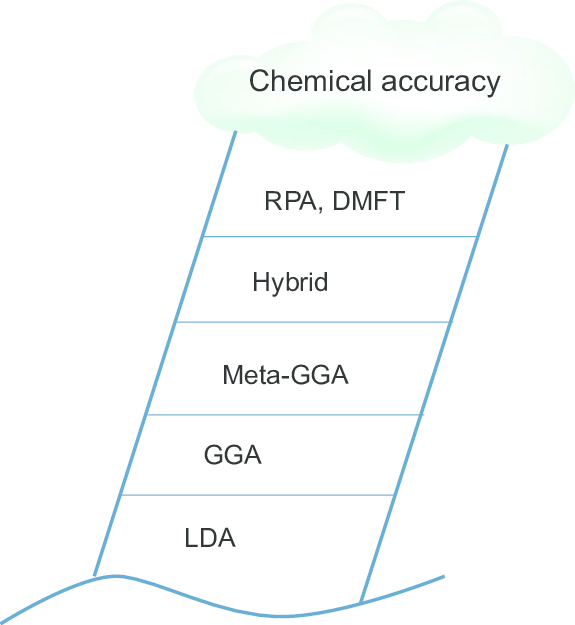
\includegraphics[width=\textwidth,height=\textheight,keepaspectratio]{Figures/jacobs_ladder.png}
    \caption{Jacob's ladder of DFT functionals. \cite{jacobs_ladder}}
    \label{fig:jacobs_ladder}
\end{figure}

\begin{itemize}
    \item \textbf{Local Density Approximation (LDA)}: Depends only on local electron density. It is accurate for uniform electron gases, but less so for molecular systems.
    \item \textbf{Generalized Gradient Approximation (GGA)}: Incorporates density gradients to improve accuracy for molecular and solid-state systems.
    \item \textbf{Meta-GGA Functionals}:  Include kinetic energy density allowing for the capture more detailed electronic effects.
    \item \textbf{Hybrid Functionals}: Combine exact exchange from Hartree-Fock with DFT terms, providing a balance between accuracy and computational cost.
    \item \textbf{Double-Hybrid Functionals}: Incorporate virtual orbital contributions, offering high predictive accuracy.
\end{itemize}

No single functional can describe all systems with equal accuracy. Each functional represents a trade-off between computational cost and precision. The optimal choice depends on the specific system and the properties of interest. 

\subsection{B3LYP functional}

The Becke, three-parameter, Lee-Yang-Parr (B3LYP) hybrid functional is one of the most widely used in computational chemistry. As a hybrid-GGA functional on Jacob’s Ladder, B3LYP incorporates exact exchange from Hartree-Fock (HF) theory. This improves its accuracy over pure DFT approaches by reducing self-interaction errors. B3LYP strikes an effective balance between computational cost and chemical accuracy, making it suitable for a variety of applications, such as structure optimization, reaction energetics, and spectroscopic studies. 

The exchange-correlation energy in B3LYP is given by:

\begin{equation}
    E_{\text{xc}}^{\text{B3LYP}} = (1 - a) E_{\text{x}}^{\text{LDA}} + a E_{\text{x}}^{\text{HF}} + b \Delta E_{\text{x}}^{\text{B88}} + (1 - c) E_{\text{c}}^{\text{LDA}} + c E_{\text{c}}^{\text{LYP}}
\end{equation}

\begin{enumerate}
    \item $E_{\text{x}}^{\text{LDA}}$ and $E_{\text{c}}^{\text{LDA}}$ are the exchange and correlation energy contributions from the Local Density Approximation (LDA).
    \item $E_{\text{x}}^{\text{HF}}$ is the exact exchange energy from Hartree-Fock theory.
    \item $\Delta E_{\text{x}}^{\text{B88}}$ is the gradient-corrected exchange functional developed by Becke (B88).
    \item $E_{\text{c}}^{\text{LYP}}$ is the correlation functional by Lee, Yang, and Parr (LYP).
    \item The parameters $a$, $b$, and $c$ are empirically optimized to improve agreement with experimental data.
\end{enumerate}

B3LYP is effective for geometry optimization, vibrational frequency calculations, thermochemistry, and TD-DFT-based excited-state studies. However, it has several limitations, such as its poor treatment of dispersion interactions and inadequate description of strong correlation effects (e.g., in transition metal complexes). Additionally, it exhibits inaccuracies in long-range charge-transfer excitations due to its incorrect asymptotic exchange behavior. B3LYP functional also tends to over-delocalize electron density in large systems. Despite these limitations, B3LYP remains widely used due to its relatively low computational cost, and many studies have reported results obtained using this functional. 


\subsection{M06-2X functional}

The M06-2X functional, developed by Zhao and Truhlar \cite{Zhao2008}, is a meta-hybrid generalized gradient approximation (meta-hybrid GGA) functional. Designed to improve the description of noncovalent interactions, thermochemistry, and reaction barriers, it is particularly useful when dispersion forces play a significant role. Compared to conventional hybrid functionals, such as B3LYP, M06-2X incorporates a higher fraction of HF exchange (54\%), enhancing its accuracy in describing main-group chemistry and long-range interactions. 

The exchange-correlation energy of M06-2X is expressed as: 

\begin{equation}
    E_{\text{xc}}^{\text{M06-2X}} = E_{\text{x}}^{\text{HF}} + (1 - a) E_{\text{x}}^{\text{GGA}} + a E_{\text{x}}^{\text{Meta-GGA}} + (1 - b) E_{\text{c}}^{\text{GGA}} + b E_{\text{c}}^{\text{Meta-GGA}}
\end{equation}

where:
\begin{enumerate}
  \item $E_{\text{x}}^{\text{HF}}$ and $E_{\text{x,LR}}^{\text{HF}}$ is the exact HF exchange,
  \item remaining terms represent exchange and correlation contributions from GGA and meta-GGA components.
  \item The parameters $a$ and $b$ were optimized through extensive benchmarking.
\end{enumerate}

M06-2X provides superior performance for systems dominated by noncovalent interactions and dispersion forces. This makes it valuable for biomolecular simulations, van der Waals complexes, and supramolecular assemblies. It also improves the prediction of reaction barriers and enhances the description of charge-transfer excitations in TD-DFT. The functional performs well in both main-group and organometallic chemistry, yielding improved bond dissociation energies, ionization potentials, and electron affinities. 

However, M06-2X has limitations as well. Its performance with transition metal complexes is inconsistent due to challenges in accurately capturing d-electron correlation. Although the high proportion of HF exchange reduces self-interaction errors, it does not eliminate them entirely. Additionally, M06-2X functional is more computationally demanding than traditional hybrid functionals and may overestimate reaction barriers in systems with strong correlation effects. Double-hybrid functionals (e.g., ωB97X-2) or dispersion-corrected methods (e.g., B3LYP-D3) may be more  accurate in such cases. 


\subsection{$\omega$B97X-D functional}

The ωB97X-D functional is a range-separated hybrid density functionals that incorporates long-range corrected exchange and empirical dispersion corrections. It was developed to overcome the limitations of traditional hybrid functionals in systems where long-range electron correlation and dispersion forces are crucial. Compared to M06-2X, which is a meta-hybrid GGA, ωB97X-D uses an explicit range-separation parameter to treat short- and long-range interactions separately. This approach is particularly well-suited for modeling extended molecular systems, such as PFAS aggregates. 

The exchange-correlation energy in ωB97X-D is expressed as: 

\begin{equation}
    E_{\text{xc}}^{\omega\text{B97X-D}} = E_{\text{x,SR}}^{\text{HF}} + (1 - a)E_{\text{x,SR}}^{\text{DFT}} + E_{\text{x,LR}}^{\text{HF}} + E_{\text{c}}^{\text{DFT}} + E_{\text{disp}}
\end{equation}

where:
\begin{enumerate}
  \item $E_{\text{x,SR}}^{\text{HF}}$ and $E_{\text{x,LR}}^{\text{HF}}$ are short- and long-range Hartree-Fock exchange.
  \item $E_{\text{x,SR}}^{\text{DFT}}$ is the short-range DFT exchange.
  \item $E_{\text{c}}^{\text{DFT}}$ is the DFT correlation energy.
  \item $E_{\text{disp}}$ is the empirical dispersion correction (Grimme's D2 model).
\end{enumerate}

Unlike B3LYP, which uses fixed HF exchange, or M06-2X, which is parameterized for main-group chemistry, ωB97X-D’s range separation improves accuracy for systems dominated by long-range electrostatics and dispersion forces. This makes it particularly well-suited for modeling weakly interacting species, such as PFAS in aqueous environments. It reduces self-interaction errors and delivers consistent performance across a wide range of molecular sizes. 

For PFAS, which feature polar C–F bonds, hydrophobic tails, and strong solvation effects, ωB97X-D offers several key advantages. Its long-range correction enhances the accuracy of hydrogen bonding; the D2 dispersion correction effectively captures noncovalent aggregation and hydrophobic interactions; and the range-separated exchange improves the modeling of charge redistribution at interfaces. Additionally, HF exchange helps mitigate self-interaction errors in PFAS systems involving electron transfer or ionization processes. 

Although ωB97X-D is more computationally demanding than B3LYP, it often achieves faster convergence than M06-2X for large systems, where self-interaction errors can hinder SCF convergence. However, ωB97X-D lacks the meta-GGA flexibility of M06-2X for modeling transition-state barriers.

\section{Computational tools and workflow}

 The initial 3D structures were generated in Avogadro \cite{avogadro2012}, using the MMFF94 force field for rapid preliminary geometry optimization \cite{avogadro_mmff94}. These pre-optimized geometries were exported as Gaussian 09 input files and processed on laboratory computers at the University of Gdańsk. Each molecule underwent full geometry optimization and vibrational frequency analysis in an aqueous solution using the PCM–SCRF solvation model \cite{gaussian_scrf}. A custom Python script was used to parse the Gaussian log files, extract energies and convert the optimized geometries into XYZ format. Solvent-accessible surface area (SASA) was computed with Open Babel \cite{oboyle2011}, and the molecular descriptors LogP and TPSA were estimated using RDKit \cite{rdkit}. The entire workflow produced nine distinct datasets, resulting from the combination of three functionals and three basis sets.

\subsection{Statistical analysis: ANOVA testing}

A two-way analysis of variance (ANOVA) was performed to evaluate the influence of different computational parameters on molecular descriptors. ANOVA is a statistical technique that determines whether there are statistically significant differences between the means of multiple groups by comparing the variance within groups to the variance between groups. In this master’s thesis, ANOVA was applied to assess the effects of the basis set and functional on the values of the calculated descriptors, as well as their interaction \cite{Orosz2022, Kovacs2021}.

\section{Used molecular descriptors}

\subsection{HOMO, LUMO and the HOMO–LUMO Gap}
The energies of the highest occupied molecular orbital (HOMO) and the lowest unoccupied molecular orbital (LUMO), and especially their difference (the gap), provide insight into a molecule’s propensity to participate in electron transfer or reactive processes. A stabilized HOMO (i.e., lower energy) indicates that the molecule is less likely to donate electrons (i.e., harder to oxidize), while a stabilized LUMO (i.e., higher energy) suggests a reduced ability to accept electrons (i.e., harder to reduce). In PFAS research, molecules with larger HOMO-LUMO gaps tend to be more resistant to oxidative or reductive degradation, which correlates with longer environmental or biological half-lives.\cite{EPA2023}.

\subsection{Topological polar surface area}

Topological polar surface area (TPSA) is calculated as the sum of the surface areas contributed by polar atoms, such as oxygen and nitrogen. Higher TPSA is associated with reduced passive membrane permeability, which may lower absorption but also slow distribution into nonpolar tissues. TPSA also influences elimination and protein binding, especially in PFAS, where high polarity affects interactions with serum proteins and clearance rates.\cite{Ryu2024}

\subsection{Dipole moment}

The molecular dipole moment reflects a molecule’s overall polarity and influences its interactions with water and polar biomolecules. PFAS with larger dipole moments tend to bind more strongly to proteins, such as serum albumin. This binding can slow renal clearance and extend the biological half-life of PFAS. \cite{PengXu2024}

\subsection{Octanol–water partition coefficient}

Octanol–water partition coefficient (LogP) describes a compound’s lipophilicity, or its tendency to partition into hydrophobic environments. In PFAS, higher LogP values are linked to greater accumulation in fatty tissues and sediments, resulting in longer biological and environmental half-lives. \cite{Qiu2020}

\subsection{Solvent accessible surface area}

Solvent accessible surface area (SASA) measures the extent of a molecule’s surface accessible to solvents, reflecting its molecular size and shape. Larger or bulkier PFAS typically exhibit greater resistance to enzymatic or microbial degradation and are metabolized more slowly \textit{in vivo}, contributing to increased persistence. In this master’s thesis, SASA values were calculated using a probe radius of 1.4Å to mimic water as the solvent. 

\subsection{Chemical hardness ($\eta$) and chemical softness ($\sigma$)}
Chemical hardness ($\eta$) is defined as half of the HOMO–LUMO gap and quantifies a molecule’s resistance to changes in electron number. The inverse of hardness, softness ($\sigma$), reflects a molecule’s susceptibility to electron exchange. Hard molecules are less reactive and more resistant to degradation pathways, while softer PFAS may react more readily and degrade more quickly.

\subsection{Chemical potential (\(\mu\)) and electrophilicity (\(\omega\))}
Chemical potential (µ), defined as the average of the HOMO and LUMO energies represents a molecule’s tendency to attract electrons. The electrophilicity index (ω), calculated as  \[
\omega = \frac{\mu^2}{2\eta}
\] quantifies a molecule’s ability to accept electrons. These descriptors, along with hardness and softness were calculated for potential use in machine learning models..

\subsection{Total hartree–fock energy}

Total HF energy reflects a molecule's electronic stabilization and serves as a check to ensure geometry optimizations have properly converged. 


%----------------------------------------------------------------------------------------
\clearpage
\section{Data set}

\subsection{Used data}\\
The primary dataset for this thesis is based on the in vivo PFAS toxicokinetic study by Dawson et al. \cite{dataset_source}. This dataset compiles biological half-life measurements structurally diverse PFAS across four mammalian species: human, monkey, rat, and mouse. Additionally, it records sex-specific differences—showing that, for certain PFAS, males exhibit longer half-lives than females. This supports the inclusion of species and sex as biological descriptors in our models.
 
These experimental data were originally used to train a binary/ranked classification model that categorized PFAS into four half-life ranges: <12h, <1 week, <2 months, and >2 months. The structural diversity of the selected PFAS ranging from short- to long-chain, and including both carboxylates and sulfonates enables robust model training and benchmarking of electronic descriptors.

For our work, we retrieved the molecular structures of nine of the studied PFAS, as well as associated species and sex labels, directly from this source. These serve as input for DFT-based descriptor calculation and subsequent machine learning model training.

The classes in the dataset correspond to biological half-life periods as follows:\\

•	Class 1 : < 0.5 day

•	Class 2: < 1 week

•	Class 3: < 2 months

•	Class 4: > 2 months

Distribution of data looks as follows
\begin{figure}[H]
    \centering
    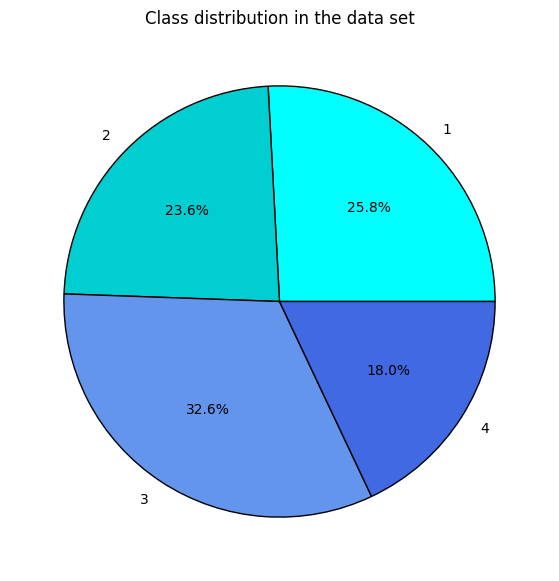
\includegraphics[width=0.5\linewidth]{Figures/classes_pie.png}
    \caption{Class distribution in the dataset}
    \label{fig:class_distribution}
\end{figure}

Figure \ref{fig:class_distribution} shows the distribution of classes within the data set. The number of com- pounds in each class is as follows:\\
•	Class 3: 27 compounds

•	Class 2: 21 compounds

•	Class 4: 16 compounds

•	Class 1: 15 compounds


\subsection{Data division}\\

The data was divided to achieve more balanced classes between the training and validation sets. Six compounds (GenX, Perfluoroheptanoic acid, Perfluorooctanoic acid, Perfluorooctanesulfonic acid, Perfluorobutanesulfonic acid, and Perfluorohexanesulfonic acid) were assigned to the training set, and three compounds (Perfluorononanoic acid, Perfluorobutanoic acid, and Perfluorodecanoic acid) to the validation set. 


Table \ref{tab:train_test_class_distribution} summarizes the distribution of compounds across the training and validation sets


\begin{table}[H]
    \centering
    \caption{Distribution of classes in training and validation set}
    \begin{tabular}{lcc}
         
 class&training set&  validation set\\
         
 3&19&  8\\
         
 2&15&  6\\
         
 4&12&  4\\
          1&11&  4\\
    \end{tabular}
    \label{tab:train_test_class_distribution}
\end{table}

\subsection{Data standarization}
To ensure that the data used in the modeling process are comparable, the next step is to standardize the data set. Standardization is essential because it gives all explanatory variables equal weight, regardless of their original measurement scales or units. Without standardization, accurately interpreting the results would be impossible. Standardization is one of the most widely applied normalization methods. As a result of this process, the data approximate a normal (Gaussian) distribution, which describes how values are distributed around the mean (Figure \ref{fig:gaussian}) \cite{GuhaR}\cite{KumarA}\cite{ZhangX}

\\

\begin{figure}[H]
    \centering
    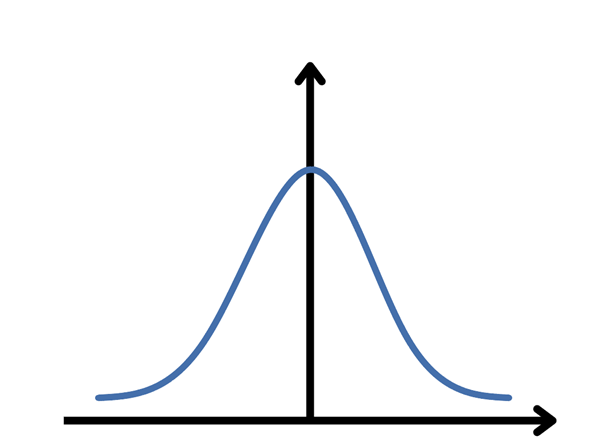
\includegraphics[width=0.5\linewidth]{Figures/image_gausian.png}
    \caption{Normal (Gaussian) distribution. The figure is for illustrative purposes only and does not represent any specific data (own work).}
    \label{fig:gaussian}
\end{figure}

Standardization is defined by the following formula:


\[
\text{z} = \frac{x - u}{\sigma}
\]
where: x - represents the sample value; u - is the mean value for all samples in the column; $\sigma$ - means the standard deviation of all the values in the column\\


In this master's thesis, data standardization was performed using the StandardScaler function from the sklearn.preprocessing library of the Python programming language.\cite{scaler}

\subsection{Feature selection}\\

As illustrated in Figure \ref{fig:heatmap_features} the descriptors were selected based on the correlation matrix, with features showing a correlation coefficient greater than 0.9 being eliminated \cite{heatmap}.

\begin{figure}[H]
    \centering
    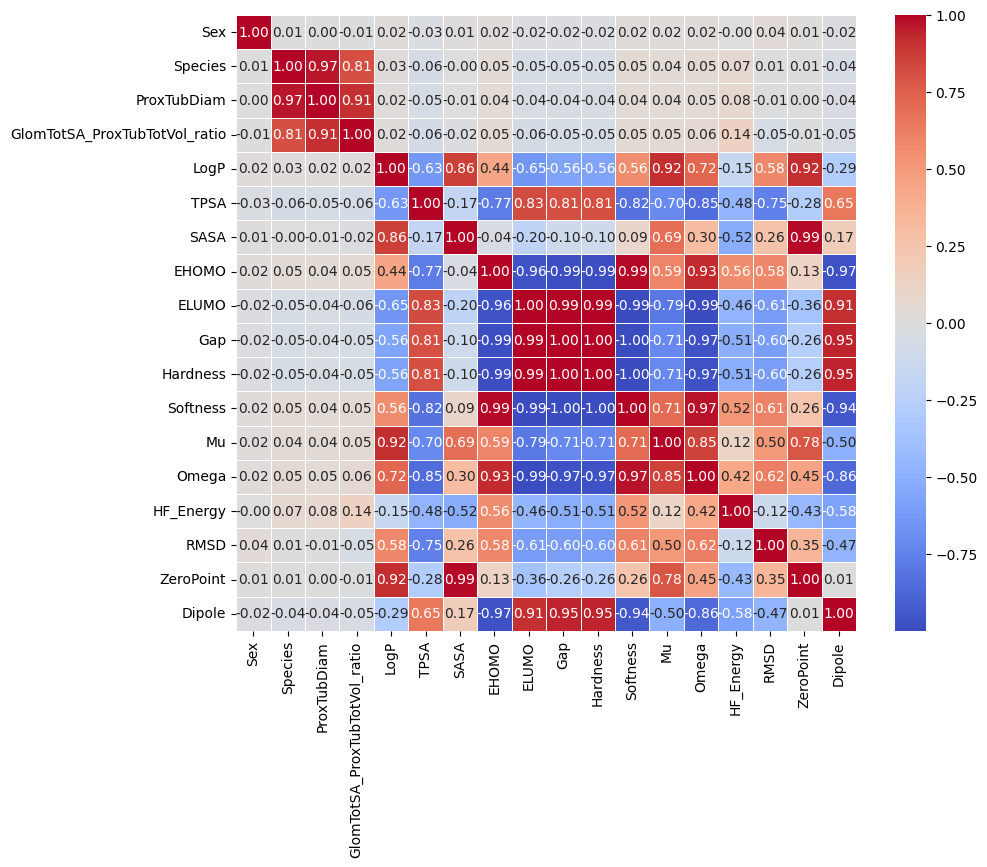
\includegraphics[width=\textwidth,height=\textheight,keepaspectratio]{Figures/matrix_corr.png}
    \caption{Correlation matrix off all features involved in analysis}
    \label{fig:heatmap_features}
\end{figure}

Accordingly, the final set of selected descriptors included the following: Sex, Species, HOMO-LUMO gap, LogP, SASA and HF energy. \textit{’Sex’} and \textit{’Species’} were categorical descriptors extracted from the source article. \cite{dataset_source}

A brief overview of each selected variables is provided below:

\begin{itemize}
    \item \textit{Sex} – This variable included two categories: \textit{‘male’} and \textit{‘female’}, which were encoded numerically as ‘0’ and ‘1’, respectively.
    
    \item \textit{Species} – This categorical variable was also transformed into numerical values: \textit{‘Mice’} = 1; \textit{‘Rats’} = 2; \textit{‘Monkeys’} = 3; and \textit{‘Human’} = 4.

    \item \textit{HOMO-LUMO Gap} – This value represents the energy gap between HOMO and LUMO.
    
    \item \textit{LogP} – This variable reflects lipophilicity, indicating a compound’s ability to dissolve in fats, oils, and nonpolar solvents.
    
    \item \textit{SASA (solvent accessible surface area)} – This molecular descriptor quantifies the surface area of a molecule accessible to a solvent. It reflects the degree to which the molecule is exposed to its surrounding environment.
    
    \item \textit{HF energy (Hartree–Fock energy)} – This descriptor represents a molecule’s total electronic energy, calculated using the Hartree–Fock method, a quantum chemical approach that provides an approximate solution to the Schrödinger equation.
\end{itemize}


\section{Machine learning methods}


\subsection{k - nearest neighbour algorithm}

The k-nearest neighbors (kNN) algorithm is a nonparametric ML method commonly used for classification and regression tasks. It works by measuring the distance between data points, typically using the Euclidean distance, which represents the straight-line distance between two points in a multidimensional space.

The modeling process begins by selecting a value for k, which specifies the number of nearest neighbors to consider. Once k is chosen, a distance matrix is calculated for all data points. Then, the algorithm identifies the k neighbors closest to the data point requiring classification. That data point is then assigned to the class that occurs most frequently among its k nearest neighbors.

For example, if k = 3, the algorithm considers the three nearest neighbors. Number of k is usually an odd number to avoid ties between classes. Suppose the point to be classified lies closest to three other points, two of them belong to class A - represented by a triangle. This class form majority among of nearest neighbors, so the point will be clafiifed as class A - triangle. (Figure \ref{fig:knn_concept}) \cite{HiranK} \cite{ChopraD}

\begin{figure}[H]
    \centering
    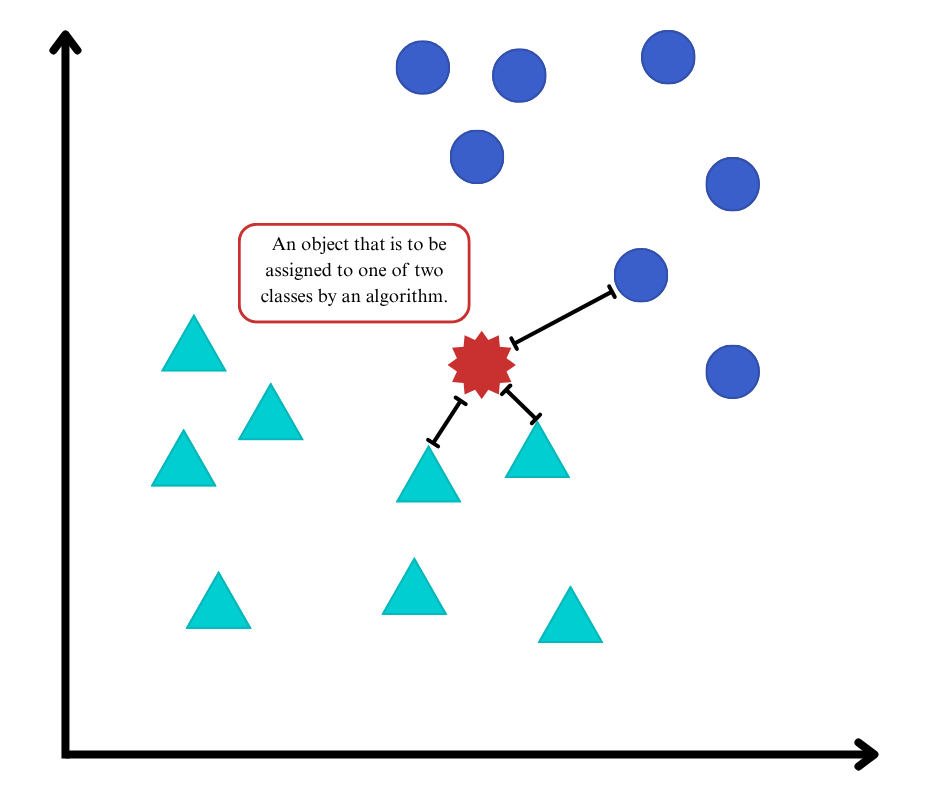
\includegraphics[width=0.5\linewidth]{Figures/knn.png}
    \caption{kNN algorithm concept. The figure is for illustrative purposes
only and does not present any specific data (own work).}
    \label{fig:knn_concept}
\end{figure}



\subsection{Decision trees}

The decision tree (DT) algorithm is a supervised ML method used for classification and regression tasks. One of its major advantages is its simplicity and easy of interpretation because it produces a tree-like diagram. However, the DT algorithm is susceptible to overfitting.

The DT algorithm partitions data along feature axes (Figure \ref{fig:dt_concept}) to accurately separate it by minimizing misclassifications at each split. After the initial division, subsequent splits are performed to further improve class separation. In the example shown, only one object (a circle) is misclassified into the triangle group.

Figure \ref{fig:dt_concept} illustrates this process using a tree structure. In a decision tree classifier, each internal node corresponds to a dataset feature, the branches denote decision rules (i.e., logical rules) based on those features, while the leaf nodes (or leaves) indicate final classification outcomes \cite{HiranK}\cite{ChopraD}.
 
\begin{figure}[H]
    \centering
    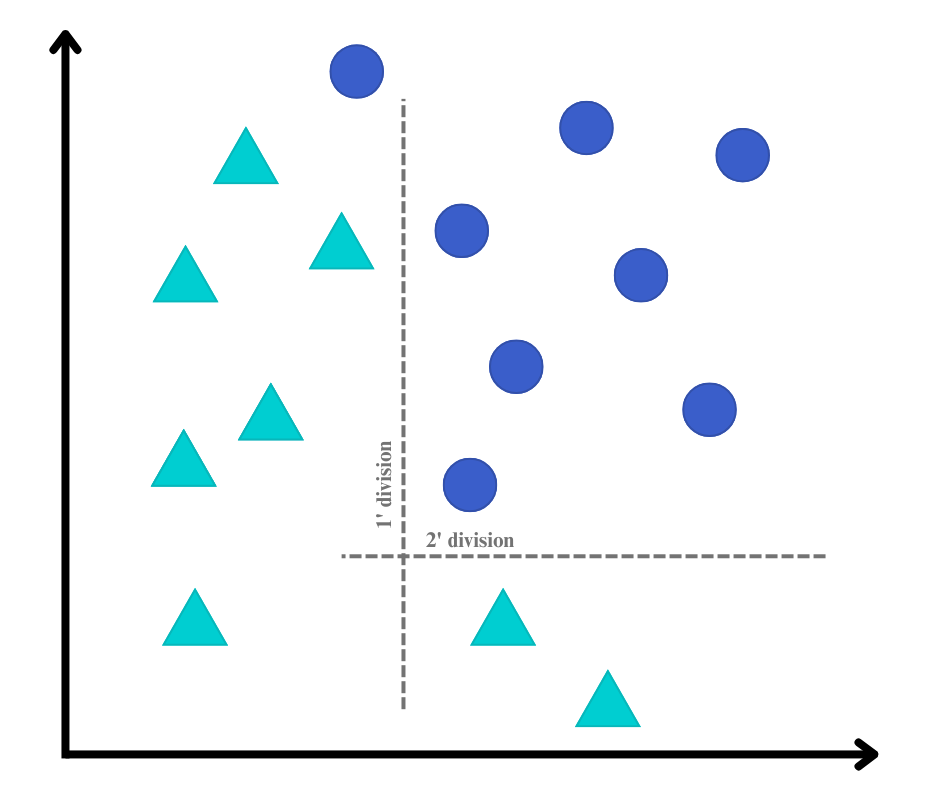
\includegraphics[width=0.5\linewidth]{Figures/DT1.png}
    \caption{The DT algorithm concept. The figure is for illustrative purposes only and does not present any specific data (own work).}
    \label{fig:dt_concept}
\end{figure}

\begin{figure}[H]
    \centering
    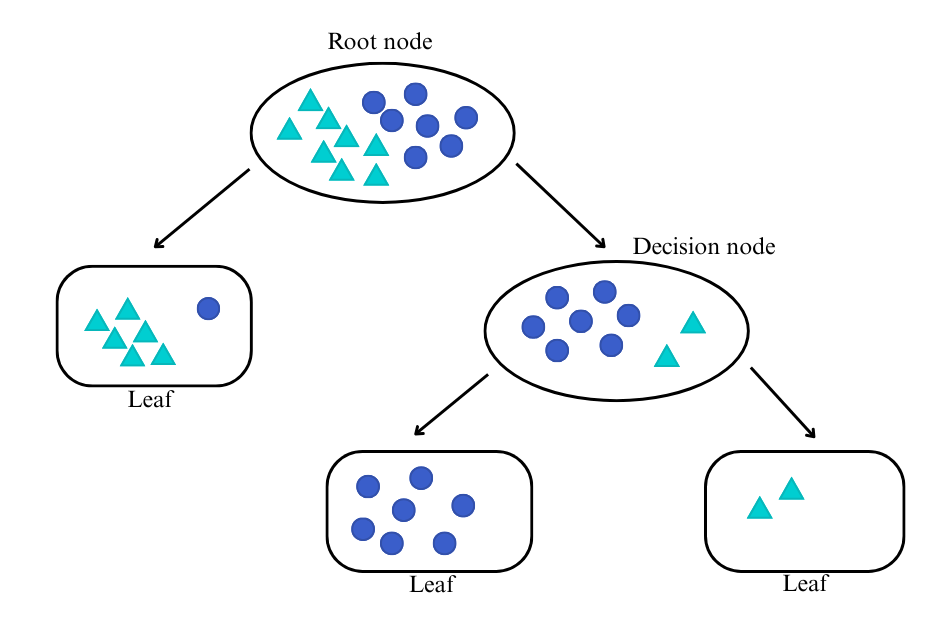
\includegraphics[width=0.5\linewidth]{Figures/DT2.png}
    \caption{The DT algorithm concept. The figure is for illustrative purposes only and does not present any specific data (own work).}
    \label{fig:enter-label}
\end{figure}


\subsection{X- gradient boosting}

XGBoost is an advanced X-gradient boosting algorithm based on DT principles. It generates an ensemble of trees sequentially, where each new tree is trained to correct the prediction errors of the preceding ones, thereby improving the model's overall performance. Despite its high accuracy, XGBoost is prone to overfitting and overtraining, especially if it is not properly regularized. XGBoost can be effectively applied to both regression and classification tasks \cite{Shah}.



\section{Evaluation metrics for classification models}

Classification model performance is assessed using a confusion matrix, which visually summarizes the number of correctly and incorrectly classified instances for each category (Figure \ref{fig:confusion_matrix}) True positive (TP) and true negative (TN) reflect accurate predictions for their respective classes. In contrast, a false positive (FP), also known as a type I error, occurs when the model incorrectly classifies a negative instance as positive. A false negative (FN), also known as a type II error, occurs when a positive instance is incorrectly classified as negative. Of these, false positives are considered more critical than false negatives. For example, in toxicity classification, misclassifying a highly toxicity compound as less toxic poses a greater risk \cite{HiranK}.
 
 
\begin{figure}[H]
    \centering
    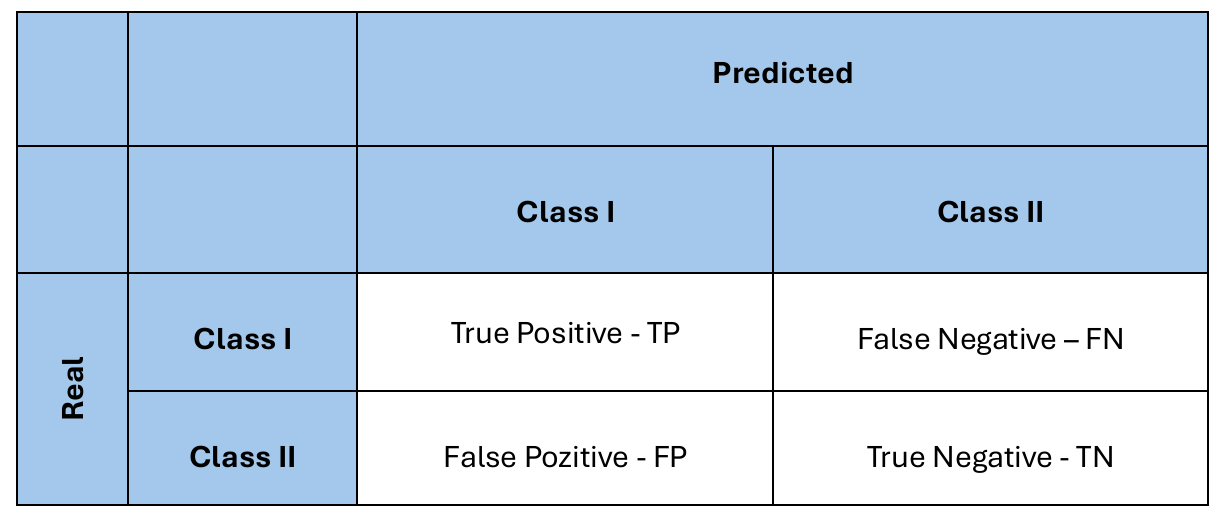
\includegraphics[width=\textwidth,height=\textheight,keepaspectratio]{Figures/matrix_conf.png}
    \caption{Confusion matrix.}
    \label{fig:confusion_matrix}
\end{figure}

The following statistics are commonly calculated using a confusion matrix:\\

I. Accuracy defines the ratio of correctly classified objects to the total number of objects \cite{HiranK}:

\[
\text{Accuracy} = \frac{TP + TN}{TP + TN + FP + FN}
\]\\

\clearpage
II. Precision defines the ratio of correctly classified true positives to all classified positives (i.e., the sum of true positives and false positives) \cite{HiranK}:

\[
\text{Precision} = \frac{TP}{TP + FP}
\]\\

III. Recall defines the ratio of correctly classified true positives to all actual positives (i.e., the sum of true positives and false negatives) \cite{HiranK}:

\[
\text{Recall} = \frac{TP}{TP + FN}
\]\\

IV. Specificity defines the ratio correctly classified true negatives to all actual negatives (i.e., the sum of true negatives and false positives) \cite{HiranK}:
\[
\text{Specificity} = \frac{TN}{TN + FP}
\]\\

V. F1-Score defines the harmonic mean of precision and recall \cite{HiranK}:

\[
\text{F1} = 2*\frac{Precision * Recall}{Precision + Recall}
\]\\


\section{Applicability domain assessment}

In the context of quantitative structure–activity/property relationship [(Q)SAR/QSPR] modeling, evaluating the applicability domain (AD) of a model is an essential step to ensure the reliability of predictions. According to the OECD guidelines for the validation of (Q)SAR models, every model should be accompanied by a clearly defined AD \cite{OECD2004}. The AD is the theoretical chemical space for which the model is expected to make reliable predictions, and compounds outside this domain may lead to extrapolation and reduced predictive accuracy.

Despite the recognized importance of AD assessment in modeling studies, the primary objective of this thesis is not to develop and validate a predictive model. Rather, the goal is to investigate the influence of various quantum-chemical descriptors computed using different exchange-correlation functionals and basis sets on compound representation and modeling performance. Therefore, in accordance with OECD recommendations, but with consideration of the scope of this work, AD will not be analyzed in detail or used as a filtering or evaluation criterion in this study.

% % Chapter 4

% \chapter{Dataset}

% \label{Chapter4}



% %----------------------------------------------------------------------------------------

% \newcommand{\keyword}[1]{\textbf{#1}}
% \newcommand{\tabhead}[1]{\textbf{#1}}
% \newcommand{\code}[1]{\texttt{#1}}
% \newcommand{\file}[1]{\texttt{\bfseries#1}}
% \newcommand{\option}[1]{\texttt{\itshape#1}}

% %----------------------------------------------------------------------------------------
 
% Chapter 5

\chapter{Results}

\label{Chapter5}

%----------------------------------------------------------------------------------------

\newcommand{\keyword}[1]{\textbf{#1}}
\newcommand{\tabhead}[1]{\textbf{#1}}
\newcommand{\code}[1]{\texttt{#1}}
\newcommand{\file}[1]{\texttt{\bfseries#1}}
\newcommand{\option}[1]{\texttt{\itshape#1}}
\renewcommand{\figurename}{Figure.}
\renewcommand{\tablename}{Table.}

%----------------------------------------------------------------------------------------

\section{Descriptor definitions and general trends}

The dataset consists of various physicochemical and quantum-chemical descriptors calculated for nine fluorinated compounds. The analyzed descriptors include: (1) the n-octanol/water partition coefficient (LogP); (2) topological polar surface area (TPSA); (3) solvent-accessible surface area (SASA); (4-5) frontier orbital energies (EHOMO and ELUMO); (6) HOMO–LUMO gap; (7) Chemical hardness ($\eta$); (8) chemical softness ($\sigma$); (9) chemical potential (μ); (10) electrophilicity index (ω); (11) total Hartree–Fock energy (HF Energy); and (12) molecular dipole moment. These properties were computed using three following basis sets: 6-31G(d,p), 6-31++G(d,p), and cc-pVTZ and three exchange-correlation functionals, namely: B3LYP, M06-2X, and ωB97X-D. For each method combination, the computational time was recorded to evaluate the balance between and descriptor precision and computational cost.

Among all the descriptors, TPSA remained consistent regardless of the computational method used (Figure. \ref{plot_tpsa}). Carboxylic acid derivatives uniformly exhibited a TPSA value of 63.0Å$^2$, which corresponds to the presence of a single carboxylate group. In comparison, sulfonic acids exhibited a higher TPSA value of 94.5Å$^2$, which was attributed to the presence of additional oxygen atoms bounded to the sulfur atom. GenX, which has a sulfonamide-like functional group, displayed a TPSA of 94.5Å$^2$, indicating a polarity level comparable to sulfonates. 6:2 chlorinated polyfluorinated ether sulfonate, trade name F-53B, the most polar compound in the dataset, had a TPSA of 126.0Å$^2$, reflecting its extended aromatic system and multiple heteroatom-containing substituents.

\begin{figure}[H]
  \centering
  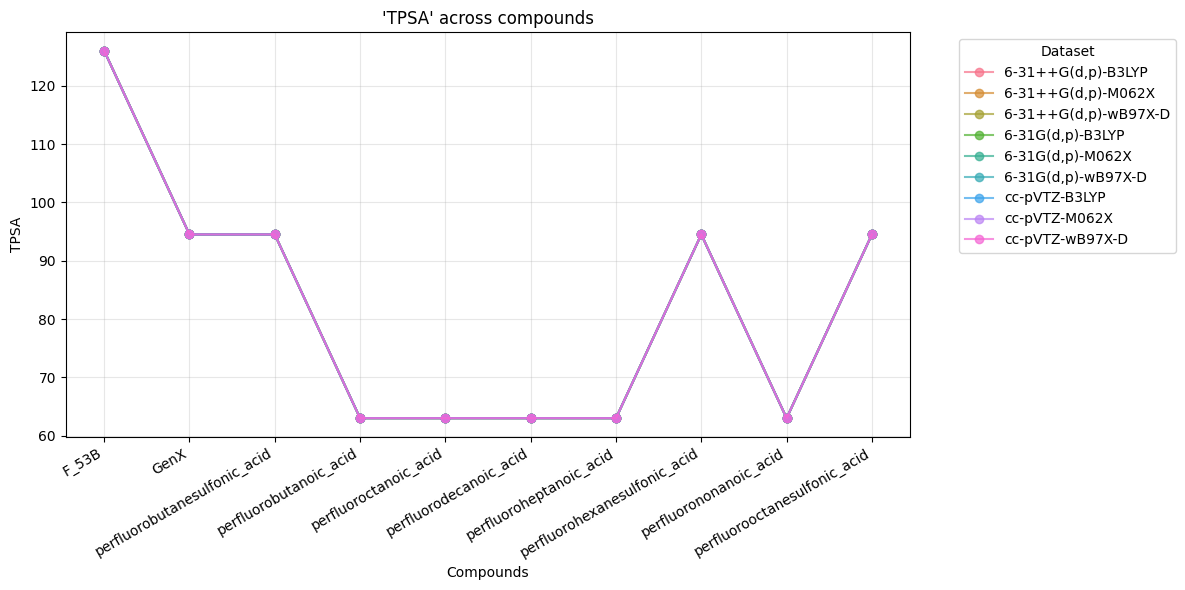
\includegraphics[width=\textwidth,height=\textheight,keepaspectratio]{Figures/plot_tpsa.png}
  \caption{Plot of topological polar surface area for each compound across all DFT methods.}
  \label{plot_tpsa}
\end{figure}

As shown in Figure. \ref{plot_sasa}, solvent-accessible surface area increases slightly when transitioning from 6-31G(d,p) to 6- 31++G(d,p), likely due to the inclusion of diffuse functions, and increases again when transitioning to cc-pVTZ. Perfluorobutanoic acid, for example, has an SASA of 164Å$^2$ at 6-31++G/B3LYP, 161Å$^2$ at 6-31G/B3LYP, and 163Å$^2$ at cc-pVTZ/B3LYP. Similar small variations are observed across all compounds. However, the general trend remains consistent: longer carbon chain correspond to proportionally larger surface area. Among the studied compounds, F53B has the largest SASA of all compounds (approximately 362Å$^2$ at 6-31++G/B3LYP and 360Å$^2$ at cc-pVTZ/B3LYP), while GenX has an intermediate SASA value (approximately 242Å$^2$ and 239Å$^2$, respectively). Sulfonic acids with carbon chain lengths comparable to those of carboxylic acids tend to exhibit slightly higher SASA values, likely due to the additional volume occupied by the sulfonate headgroup.

\begin{figure}[H]
  \centering
  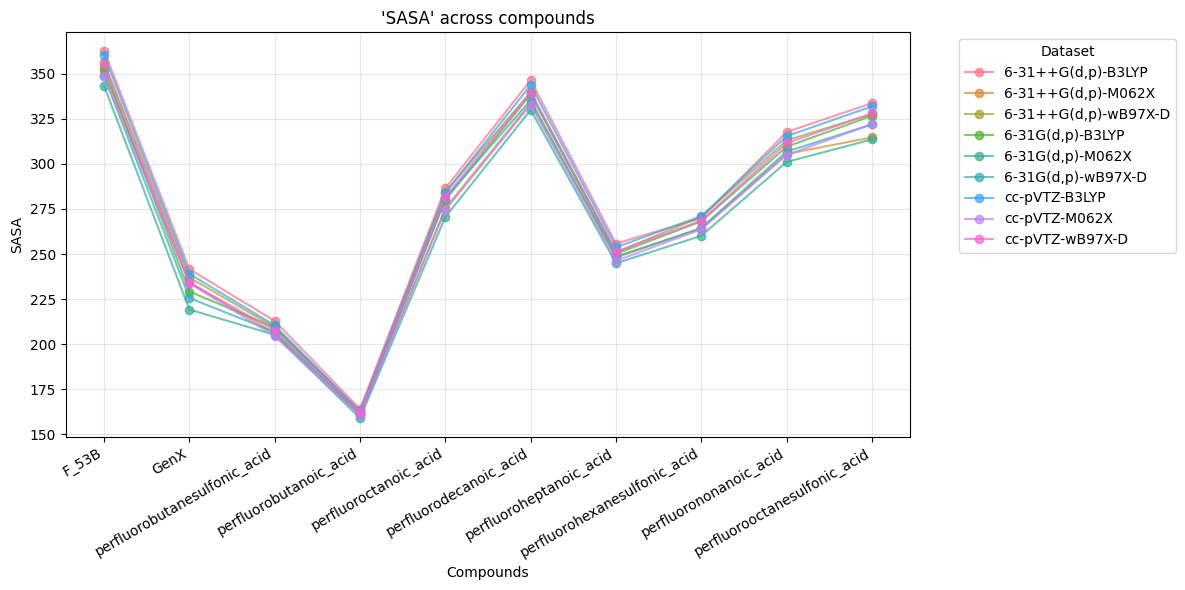
\includegraphics[width=\textwidth,height=\textheight,keepaspectratio]{Figures/plot_sasa.png}
  \caption{Plot of solvent accessible surface area (1.4Å water molecule probe) for each compound across all DFT methods.}
  \label{plot_sasa}
\end{figure}


\subsection{Frontier orbital energies and reactivity indices}

The energies of the highest occupied (HOMO) and lowest unoccupied (LUMO) molecular orbitals depend on the functional and basis set used (Figure \ref{plot_homo} and Figure \ref{plot_lumo}). However, clear trends emerge across different PFAS classes. Sulfonates and F53B consistently have more stable (i.e., lower) HOMO energies than carboxylates, indicating lower susceptibility to oxidation. Similarly, their LUMO energies are generally higher, indicating reduced electron affinity and a lower likelihood of undergoing reductive transformations.

\begin{figure}[H]
  \centering
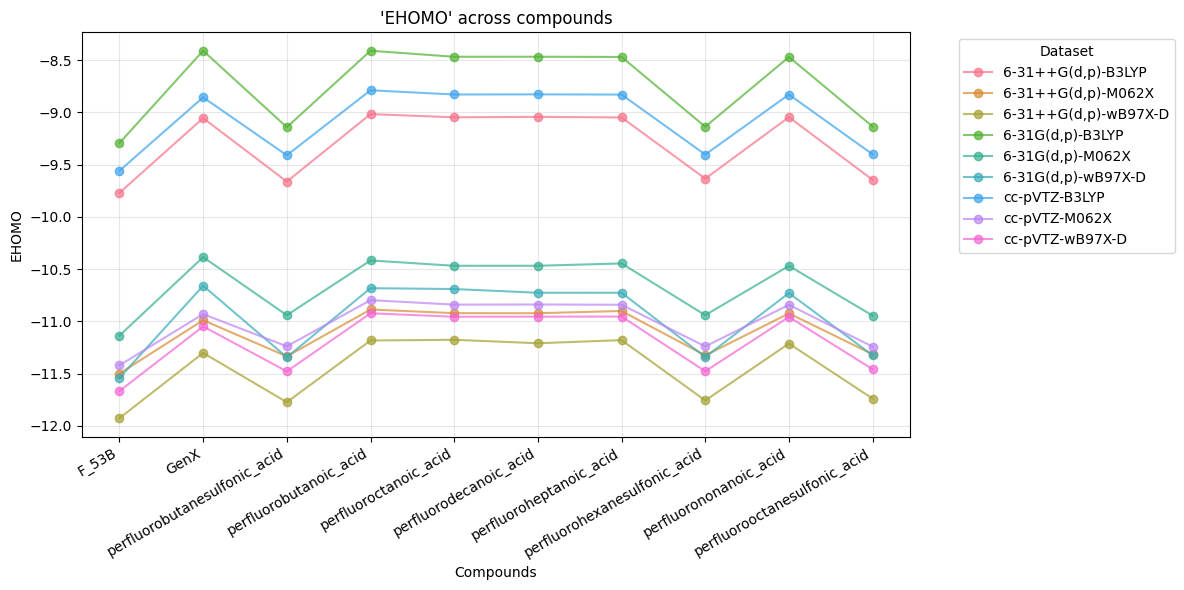
\includegraphics[width=\textwidth,height=\textheight,keepaspectratio]{Figures/plot_homo.png}
  \caption{Plot of HOMO energy for each compound across all DFT methods.}
  \label{plot_homo}
\end{figure}

\begin{figure}[H]
  \centering
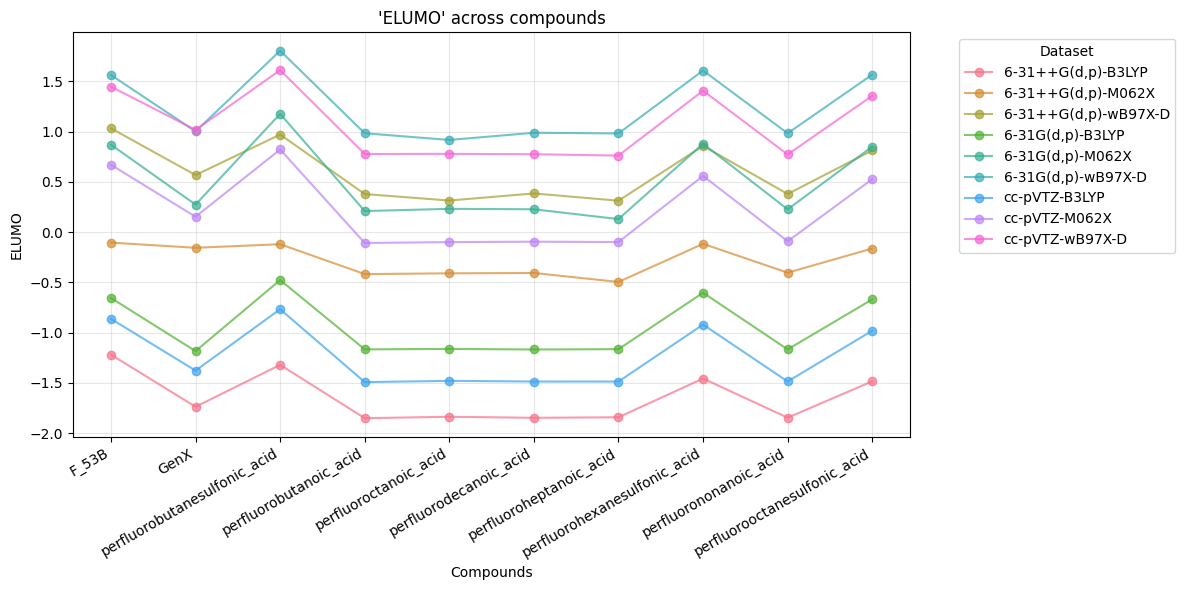
\includegraphics[width=\textwidth,height=\textheight,keepaspectratio]{Figures/plot_lumo.png}
  \caption{Plot of LUMO energy for each compound across all DFT methods.}
  \label{plot_lumo}
\end{figure}

The HOMO–LUMO gap, a key indicator of kinetic stability, is larger for sulfonates and F53B than for carboxylates (Figure \ref{plot_gap}). This suggests that these compounds are more chemically stable, consistent with their persistence in the environment and human body. GenX typically falls between these two groups, reflecting its hybrid structure.

\begin{figure}[H]
  \centering
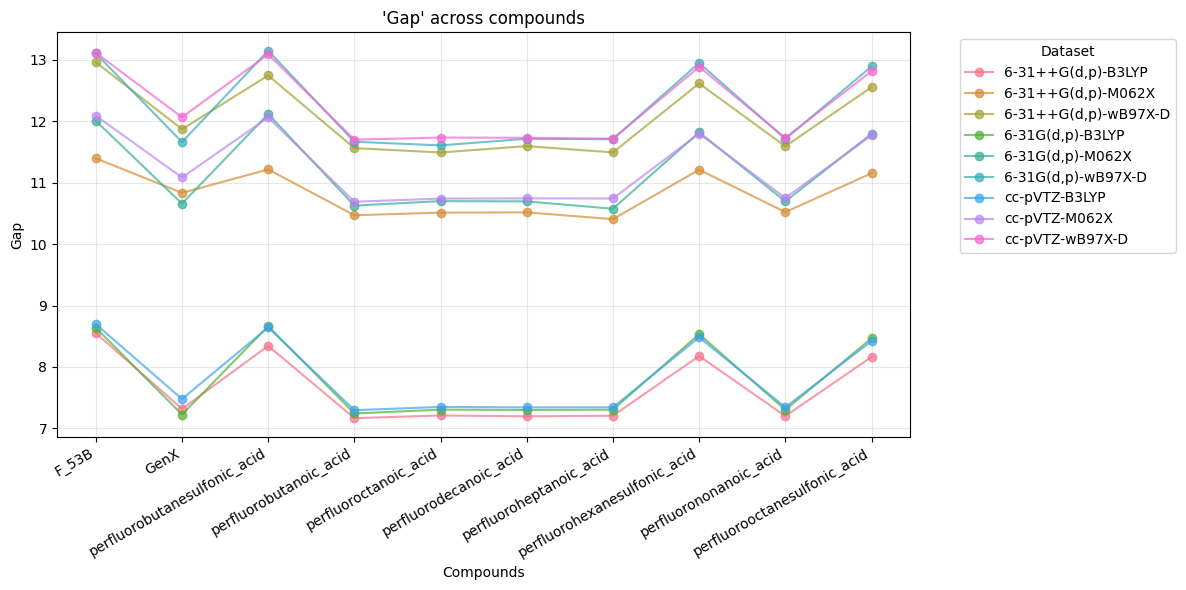
\includegraphics[width=\textwidth,height=\textheight,keepaspectratio]{Figures/plot_gap.png}
  \caption{Plot of HOMO-LUMO gap for each compound across all DFT methods.}
  \label{plot_gap}
\end{figure}

\begin{figure}[H]
  \centering
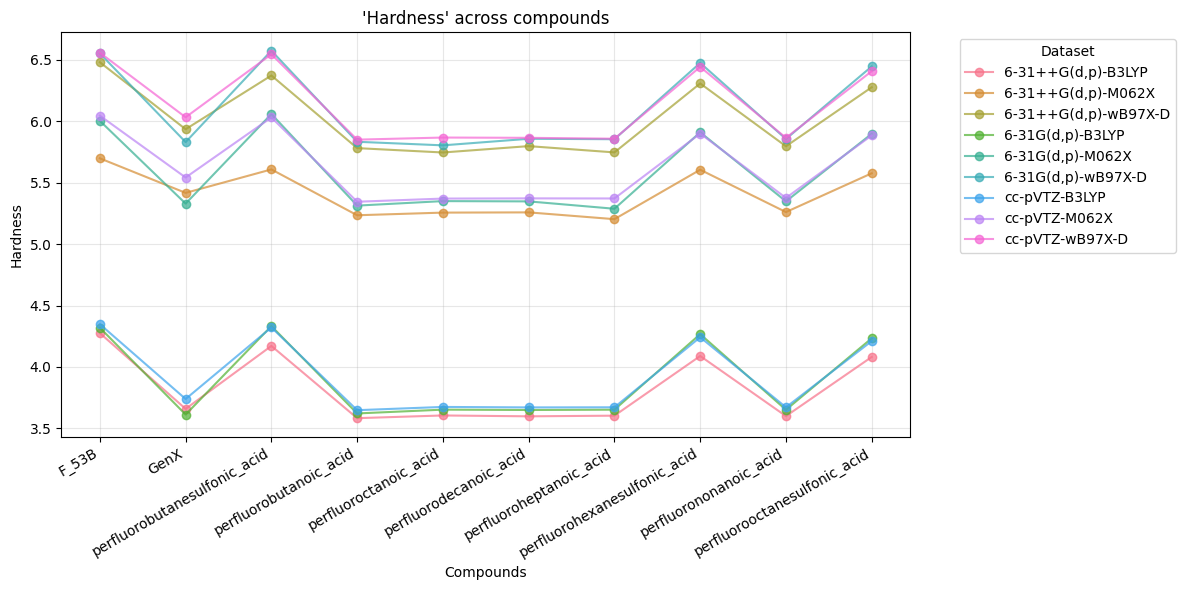
\includegraphics[width=\textwidth,height=\textheight,keepaspectratio]{Figures/plot_hardness.png}
  \caption{Plot of chemical hardness for each compound across all DFT methods.}
  \label{plot_hardness}
\end{figure}

\begin{figure}[H]
  \centering
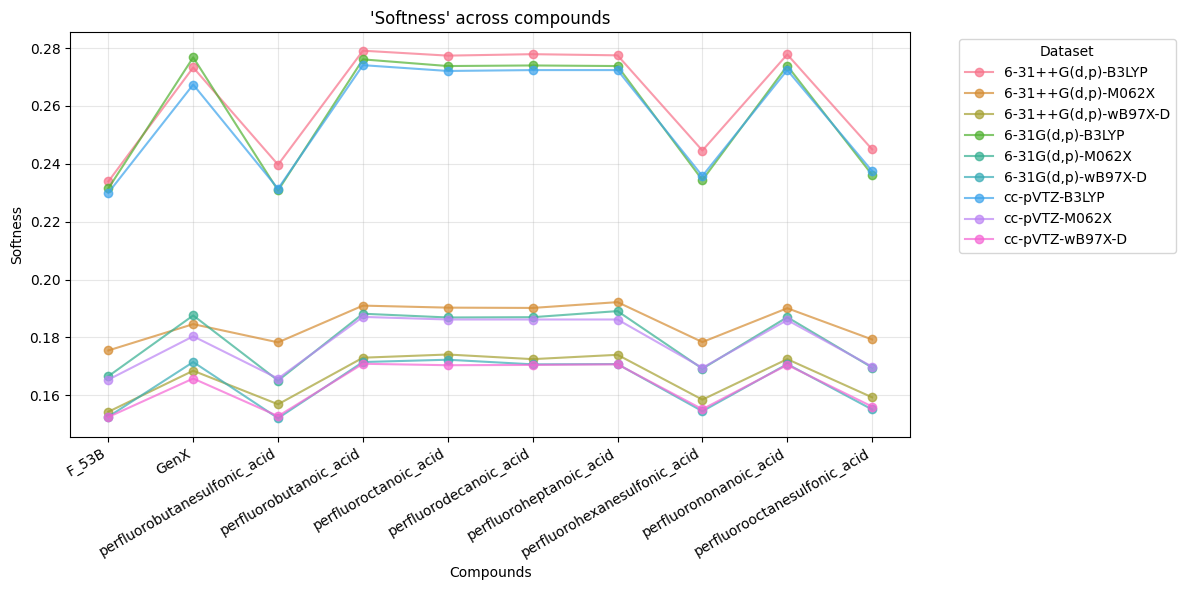
\includegraphics[width=\textwidth,height=\textheight,keepaspectratio]{Figures/plot_softness.png}
  \caption{Plot of chemical softness for each compound across all DFT methods.}
  \label{plot_softness}
\end{figure}

Similar to the HOMO–LUMO gap, chemical hardness ($\eta$) follows the similar pattern: sulfonates and F53B are harder, while carboxylates are softer and therefore more reactive (Figure \ref{plot_hardness}). This trend is important because softer, more reactive molecules tend to degrade more rapidly than harder molecules, which are generally more resistant to transformation.
Under B3LYP/6-31G(d,p), hardness for carboxylates lies around 3.6–3.7 eV, rising to ~4.1–4.3 eV for sulfonates or F53B when adding diffuse functions or moving to cc-pVTZ. Switching to M06-2X increases hardness by ~1.6–1.8 eV at each basis (e.g., perfluorobutanoic acid from ~3.58 to ~5.23 eV at 6-31++G(d,p)), and B97X-D further raises hardness by another ~0.5–0.8 eV (e.g., F53B hardness from ~4.28 eV under B3LYP/6-31++G(d,p) to ~6.48 eV under ωB97X-D/6-31++G(d,p)). Enlarging the basis from 6-31++G(d,p) to cc-pVTZ produces a modest additional increase (~0.1–0.3 eV) across functionals. Thus, both functional (more exact exchange) and larger basis sets systematically elevate hardness, reinforcing that method selection strongly influences predicted kinetic stability.  


Carboxylates, which feature lower hardness, show correspondingly higher softness, while sulfonates and F53B maintain lower softness across 3D-sensitive methods (Figure \ref{plot_softness}). Softness decreases (i.e., hardness increases) when progressing from \texttt{B3LYP} to \texttt{M06‑2X} and \texttt{$\omega$B97X‑D}, and when using larger basis sets such as \texttt{cc‑pVTZ}. For example, F53B softness drops from ~0.23 \texttt{(B3LYP/6‑31++G(d,p))} to ~0.15 \texttt{($\omega$B97X‑D/cc‑pVTZ)}, mirroring trends in gap and hardness.

\begin{figure}[H]
  \centering
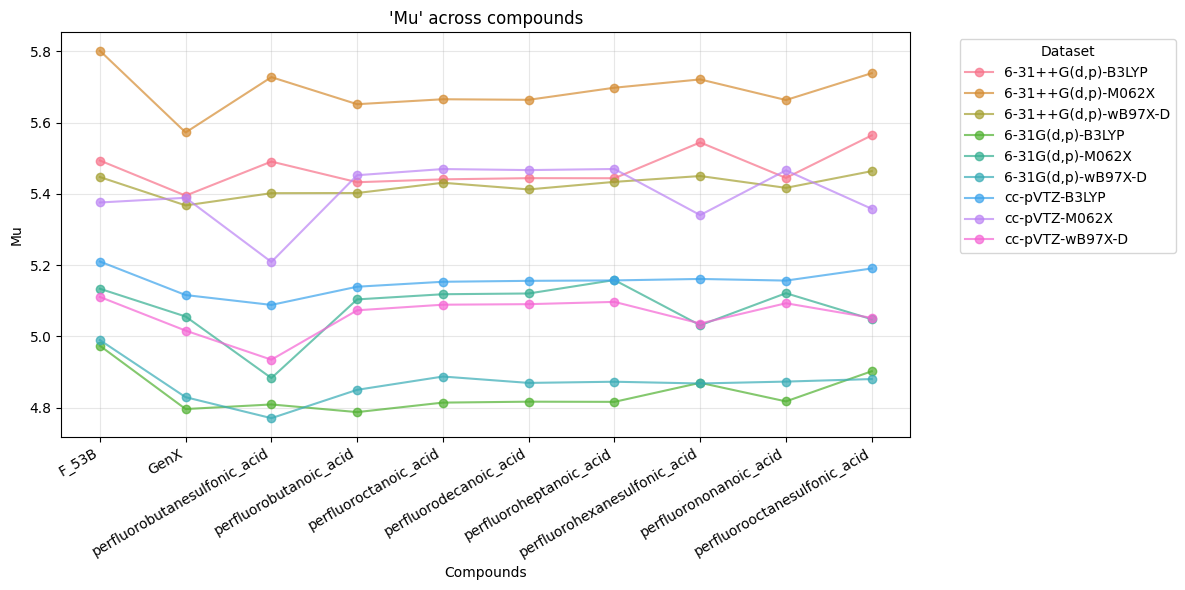
\includegraphics[width=\textwidth,height=\textheight,keepaspectratio]{Figures/plot_mu.png}
  \caption{Plot of chemical potential for each compound across all DFT methods.}
  \label{plot_mu}
\end{figure}

\begin{figure}[H]
  \centering
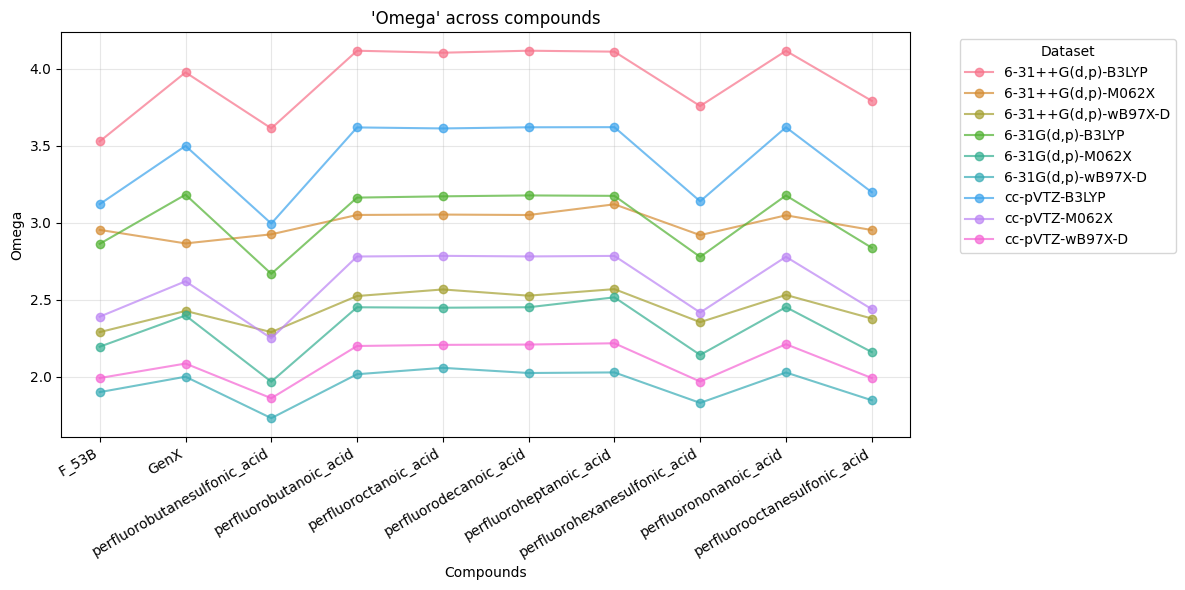
\includegraphics[width=\textwidth,height=\textheight,keepaspectratio]{Figures/plot_omega.png}
  \caption{Plot of electrophilicity index for each compound across all DFT methods.}
  \label{plot_omega}
\end{figure}

Although the chemical potential and electrophilicity index show smaller differences, they still support the same conclusion: sulfonates and F53B are somewhat less electrophilic, making them less likely to undergo reactions that could reduce their half-life (Figure \ref{plot_mu}). Chemical potential (μ) tends to be lower for B3LYP than for M06-2X, while ωB97X-D often yields values between or slightly below these, and enlarging the basis (from 6-31G(d,p) to 6-31++G(d,p) to cc-pVTZ) shifts μ modestly upward. Electrophilicity index (ω) shows a clearer downward trend when moving to higher-exact-exchange functionals and larger bases (Figure \ref{plot_omega}): B3LYP produces the highest ω, M06-2X lowers it, and ωB97X-D yields the lowest values; likewise, switching from 6-31++G(d,p) to cc-pVTZ further reduces ω. These shifts, though smaller than for gap or hardness, underscore that both functional and basis choice should meaningfully influence μ and ω magnitudes.


\subsection{Molecular dipole moments}

Molecular dipole moments are moderately sensitive to the choice of functional and the basis set (Figure \ref{plot_dipole}). At the B3LYP/6-31++G(d,p) level of theory, for example, the dipole moment of perfluorobutanoic acid is 3.93D, whereas the dipole moment of perfluoroctanoic acid is 3.18D. Perfluorobutanesulfonic acid and perfluorooctanesulfonic acid have dipole moments of 3.64D and 3.77D, respectively. GenX has a dipole of 3.30D, while F53B has a dipole of 4.64D. The inclusion of diffuse functions generally increases dipole moments by approximately 0.1–0.3D. Switching to the cc-pVTZ basis set, however, results in minor changes, typically within ±0.1D. Functionals that include a higher proportion of exact exchange, such as M06-2X and ωB97X-D, tend to yield slightly lower dipole moments than B3LYP (Figure \ref{plot_dipole}).

\begin{figure}[H]
  \centering
  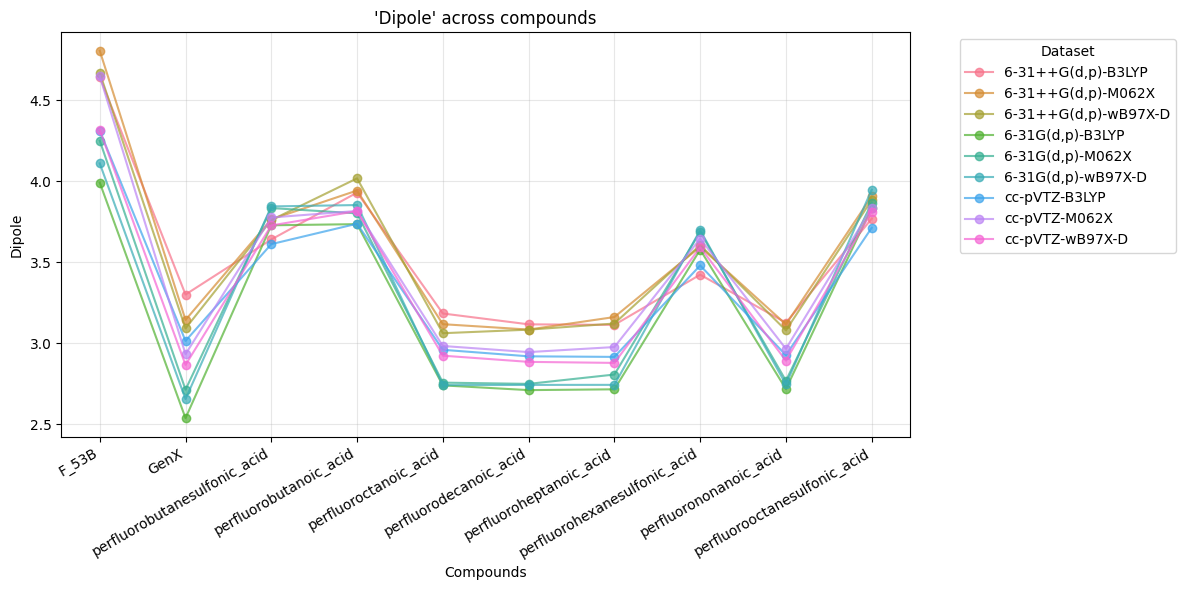
\includegraphics[width=\textwidth,height=\textheight,keepaspectratio]{Figures/plot_dipole.png}
  \caption{Plot of dipole moments for each compound across all DFT methods.}
  \label{plot_dipole}
\end{figure}


\section{Computational timing and trade-off analysis}

Calculation times increase significantly when using larger basis sets, more complex functionals, or when modeling larger molecules. For example, geometry optimization of perfluorobutanoic acid using B3LYP with the 6-31G(d,p) basis set takes approximately three minutes (Figure \ref{plot_time}). Adding diffuse functions (6-31++G(d,p)) increases computation time to around 19 minutes. Switching to the cc-pVTZ basis set increases computation time to approximately 116 minutes. For PFOA, the computation times are 27 minutes with B3LYP/6-31G(d,p), 270 minutes with B3LYP/6-31++G(d,p), and 1,291 minutes with B3LYP/cc-pVTZ. F53B the most computationally demanding molecule in this master’s project, requires 44 minutes at B3LYP/6-31G(d,p), 659 minutes at B3LYP/6-31++G(d,p), and 4980 minutes at B3LYP/cc-pVTZ.

Switching to the M06-2X functional generally increases computation times by a factor of approximately 1.2 to 1.5 for each basis set level. For instance, perfluorobutanoic acid requires five minutes at M06-2X/6-31G(d,p), 26 minutes at M06-2X/6-31++G(d,p), and 136 minutes at M06-2X/cc-pVTZ). The ωB97X-D functional is typically the most computationally intensive, increasing runtimes by an additional 20\% - 30\% compared to M06-2X for the same basis set (Figure \ref{plot_time}).

\begin{figure}[H]
  \centering
  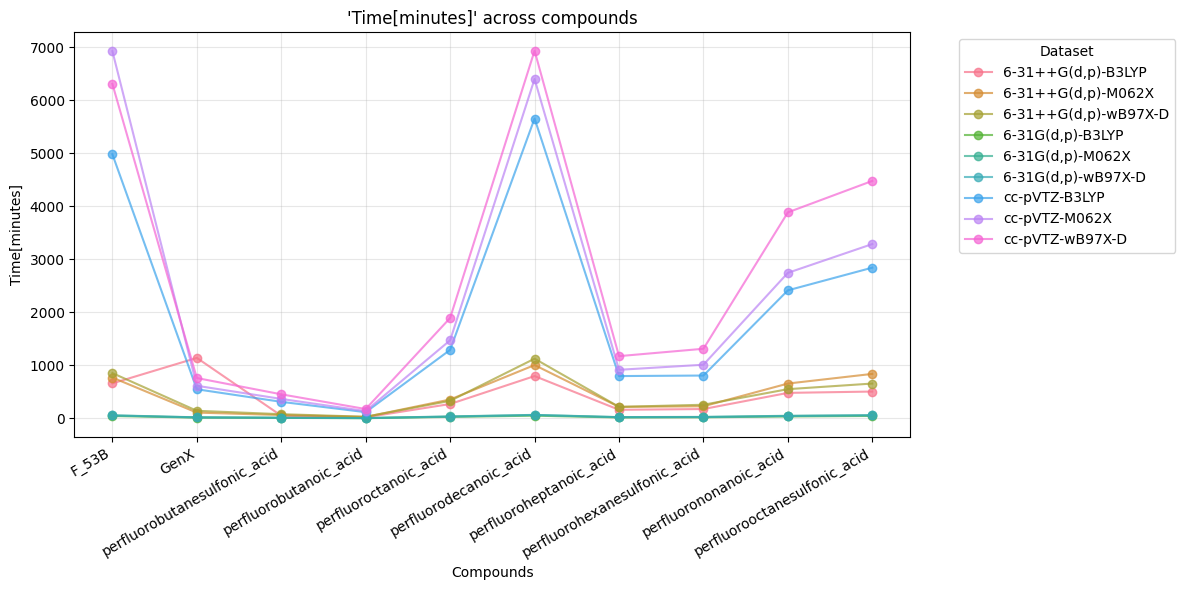
\includegraphics[width=\textwidth,height=\textheight,keepaspectratio]{Figures/plot_time.png}
  \caption{Plot of calculation time in minutes for each compound across all DFT methods.}
  \label{plot_time}
\end{figure}

Since calculation time scales approximately with the cube of the number of basis functions, longer perfluorocarbon chains, such as PFOA or PFDA, and more complex scaffolds, such as GenX or F53B, result in significantly longer runtimes at higher levels of theory. For routine descriptor generation, B3LYP combined with the 6-31G(d,p) basis set captures qualitative trends in chemical hardness, chemical softness, and orbital energies with minimal computational cost. However, accurate ELUMO values are needed for predicting reduction potentials or excited-state properties. In these cases, it is advisable to include diffuse functions (e.g., 6-31++G(d,p)) or, preferably, use a triple-ζ basis set, such as cc-pVTZ. Among the functionals tested, ωB97X-D generally provides the most reliable HOMO–LUMO gap values, albeit at the highest computational expense. M06-2X paired with 6-31++G(d,p) is a practical compromise that reproduces cc-pVTZ gap values within 0.1–0.2eV while requiring only about one-tenth of the computational time


\section{Group distinctions among PFAS, GenX, and F53B}

The perfluoroalkyl carboxylic acids (perfluorobutanoic acid, perfluorooctanoic acid, perfluorononanoic acid, perfluorodecanoic acid, and perfluoroheptanoic acid) exhibit a clear trend: as the fluorocarbon chain length increases, hydrophobicity also increases, while polar surface area and reactivity indices remain nearly constant. Regardless of the functional used, their EHOMO values cluster closely, and their electrophilicity indices fall within a narrow range.

In contrast, the perfluorosulfonic acids (perfluorobutanesulfonic acid, perfluorohexane- sulfonic acid, and perfluorooctanesulfonic acid) form a distinct group. They possess higher topological polar surface areas, slightly larger HOMO–LUMO gaps (and therefore greater chemical hardness), and correspondingly lower chemical softness compared to carboxylic acids of equivalent chain length. Their molecular dipole moments are typically 0.2–0.4D higher, and their chemical potentials are approximately 0.05–0.10eV more negative.

GenX acts as a bridges these two clusters. Its TPSA is comparable to that of sulfonates, yet its chemical hardness and softness more closely resemble those of medium-chain carboxylates. Under B3LYP/6-31++G(d,p), GenX exhibits ELUMO and EHOMO energies of –1.74eV and –9.05eV, respectively, resulting in a HOMO–LUMO gap of 7.32eV—nearly identical to that of PFOA (7.21eV). However, its dipole moment of 3.30D is slightly lower than that of PFOA (3.18D) and PFBS (3.64D). From a computational perspective, GenX requires significantly longer runtimes than PFAS molecules with comparable heavy-atom counts, due to its oxygenated and branched substituents. These increase the number of basis function and hinder convergence.

F53B is distinct from the PFCA and PFSA subgroups. It has the largest TPSA (126.0Å$^2$), the greatest dipole moment (up to 4.80D under M06-2X/6-31++G(d,p)), and the highest chemical hardness (up to 6.48eV under ωB97X-D/6-31++G(d,p)). These properties reflect its polyfunctional structure. However, F53B’s reactivity indices and polar surface area do not align cleanly with either group. The computational cost for F53B increases accordingly. At cc-pVTZ/ωB97XD, the runtime exceeds 6300 minutes (approximately 105 hours), highlighting that molecules of this complexity incur substantial computational overhead.


%----------------------------------------------------------------------------------------
\section{Influence of basis set and functional}

A two-way ANOVA was performed for each descriptor to evaluate the influence of the basis set, functional, and their interaction on computed molecular descriptors. Three levels of basis sets and three levels of functionals were used.

\clearpage
\subsection{Descriptors with no significant effects}

Neither the basis set, the functional, nor their interaction had a statistically significant effect on the following descriptors (all p > 0.05):

\begin{itemize}
    \item LogP (as value is not 3D-structure dependent)
    \item TPSA
    \item SASA
    \item HF Energy
    \item Dipole
\end{itemize}

These properties show minimal variation when different basis sets or functionals are used. This suggests that the choice of computational method does not significantly impact the results for these descriptors. Figures \ref{anova_logP}, \ref{anova_tpsa}, \ref{anova_sasa}, \ref{anova_hf} and \ref{anova_dipole} present nearly flat mean values across all combinations, confirming negligible method dependence.

\begin{figure}[H]
\centering
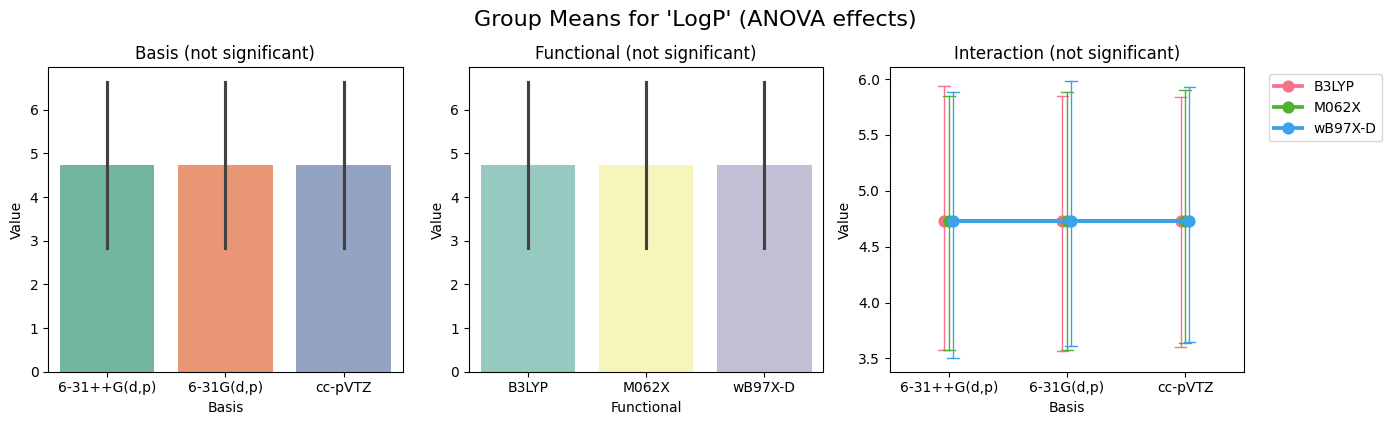
\includegraphics[width=\textwidth,height=\textheight,keepaspectratio]{Figures/anova_logP.png}
\caption{Group means for LogP. There were no significant effects observed for the basis set, the functional, or their combination.}
\label{anova_logP}
\end{figure}

\begin{figure}[H]
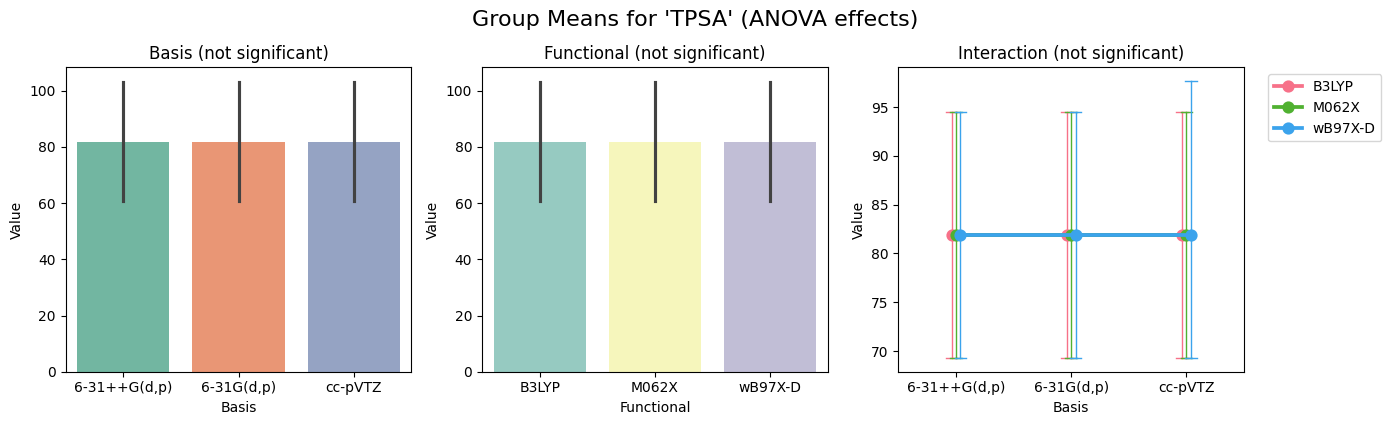
\includegraphics[width=\textwidth,height=\textheight,keepaspectratio]{Figures/anova_tpsa.png}
\caption{Group means for topological polar surface area. There were no significant effects observed for the basis set, the functional, or their combination.}
\label{anova_tpsa}
\end{figure}

\begin{figure}[H]
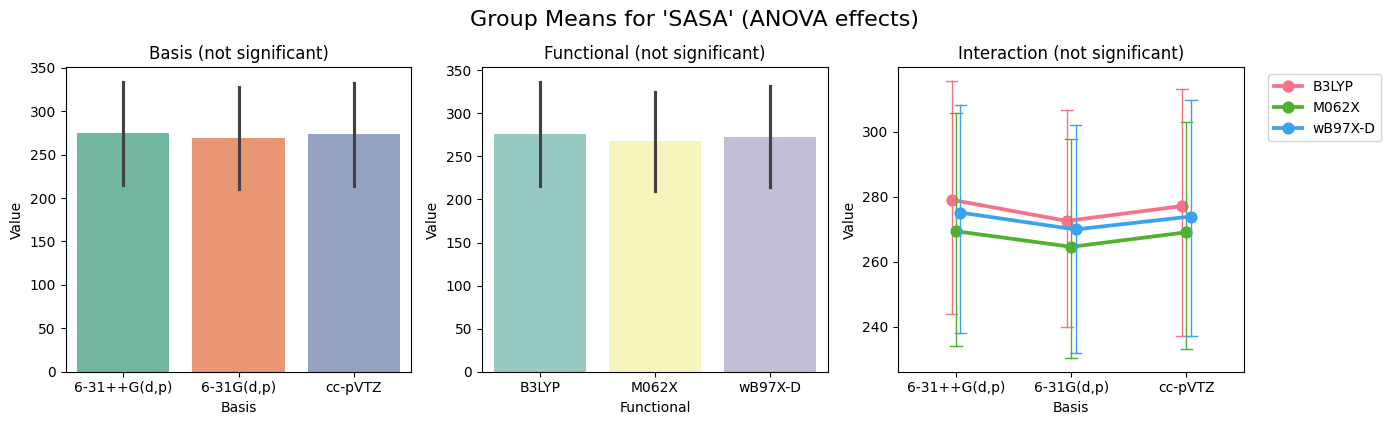
\includegraphics[width=\textwidth,height=\textheight,keepaspectratio]{Figures/anova_sasa.png}
\caption{Group means for solvent accessible surface area. There were no significant effects observed for the basis set, the functional or their combination.}
\label{anova_sasa}
\end{figure}

\begin{figure}[H]
\centering
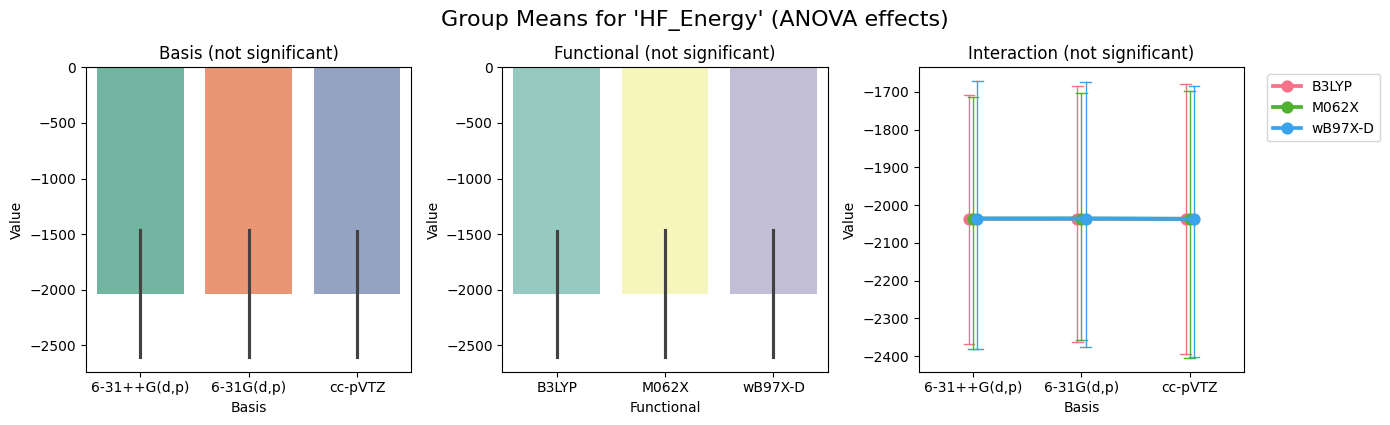
\includegraphics[width=\textwidth,height=\textheight,keepaspectratio]{Figures/anova_hf.png}
\caption{Group means for HF energy. There were no significant effects observed for the basis set, the functional or their combination.}
\label{anova_hf}
\end{figure}

\begin{figure}[H]
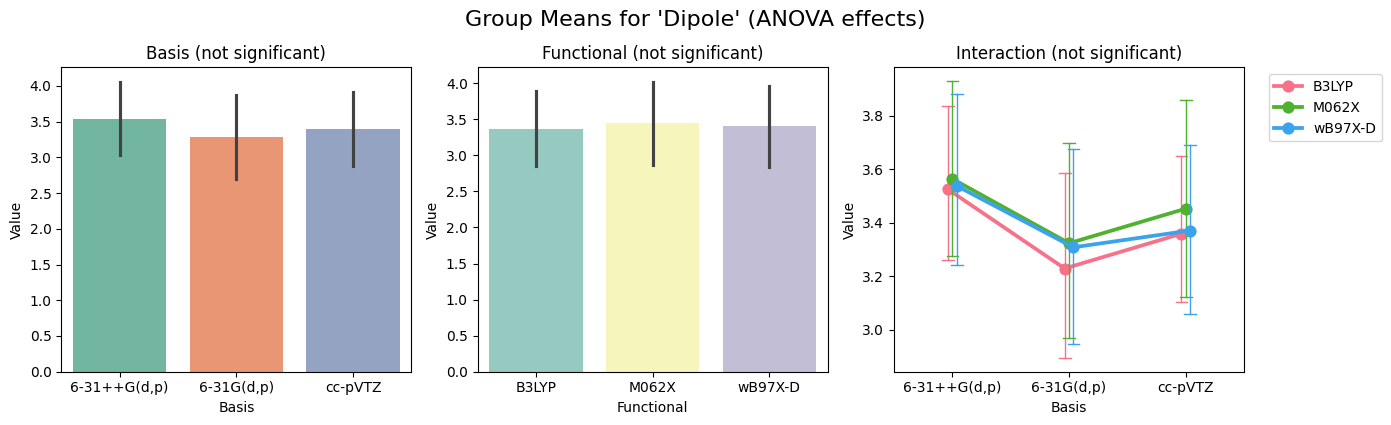
\includegraphics[width=\textwidth,height=\textheight,keepaspectratio]{Figures/anova_dipole.png}
\caption{Group means for total dipole moment. There were no significant effects observed for the basis set, the functional or their combination.}
\label{anova_dipole}
\end{figure}

\subsection{Descriptors with significant effects}
\subsection*{Descriptors with significant functional effects only}

The following descriptors and features had a statistically significant functional effect (p < 0.05), while the effects of the basis set and their interaction were not significant:

\begin{itemize}
    \item HOMO-LUMO Gap
    \item Chemical hardness
    \item Chemical softness
    \item Calculation time (not a descriptor)
\end{itemize}

\begin{figure}[H]
\centering
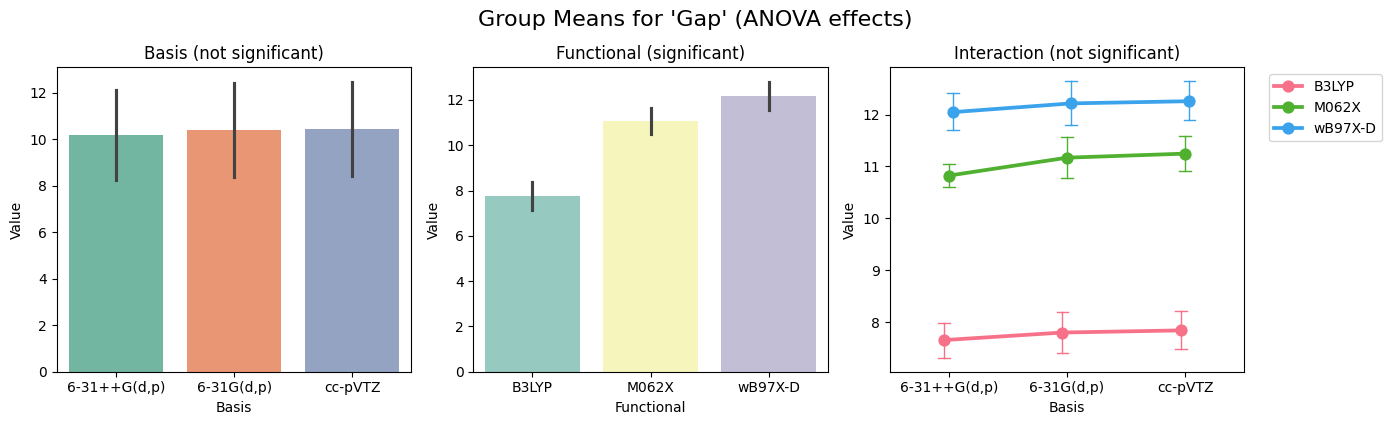
\includegraphics[width=\textwidth,height=\textheight,keepaspectratio]{Figures/anova_gap.png}
\caption{Group means for the HOMO-LUMO energy gap. The average energy gap grows with more complex functionals.}
\label{anova_gap}
\end{figure}

\begin{figure}[H]
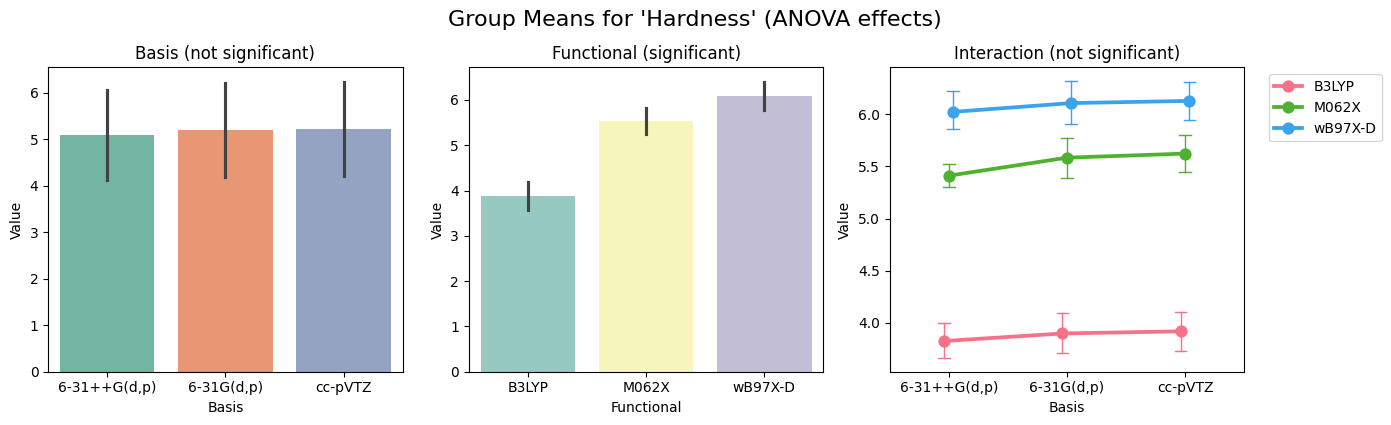
\includegraphics[width=\textwidth,height=\textheight,keepaspectratio]{Figures/anova_hardness.png}
\caption{Group means for the chemical hardness. The average chemical hardness increases with more complex functionals.}
\label{anova_hardness}
\end{figure}

\begin{figure}[H]
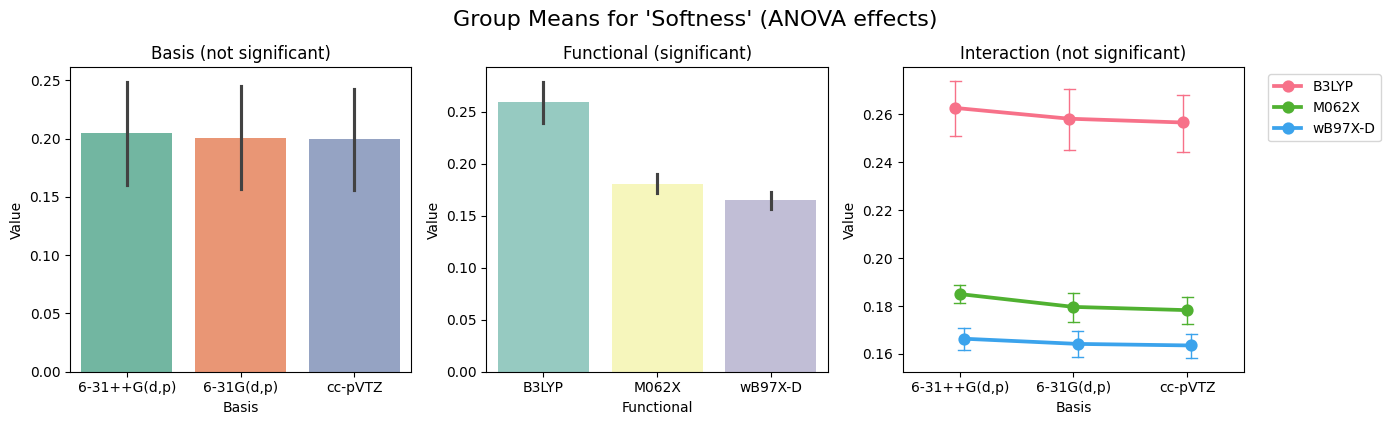
\includegraphics[width=\textwidth,height=\textheight,keepaspectratio]{Figures/anova_softness.png}
\caption{Group means for chemical softness. The average chemical hardness decreases with more complex functionals.}
\label{anova_softness}
\end{figure}

\begin{figure}[H]
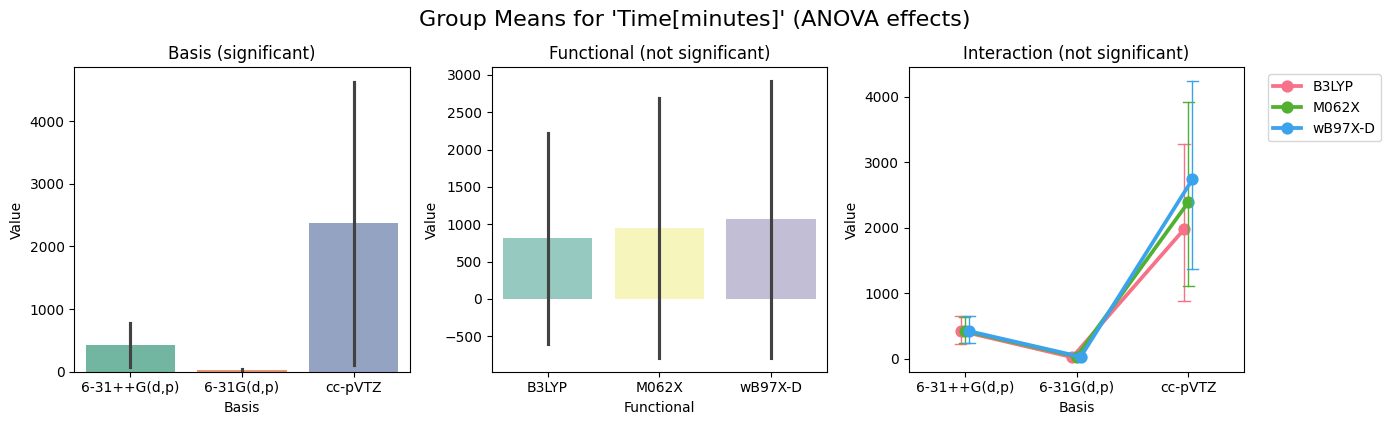
\includegraphics[width=\textwidth,height=\textheight,keepaspectratio]{Figures/anova_time.png}
\caption{Group means for time of calculation in minutes. We can see a big computational cost tradeoff with expanding basis set.}
\label{anova_time}
\end{figure}

\clearpage
The HOMO–LUMO gap varies notably across functionals (e.g., increasing from B3LYP to M06-2X to ωB97X-D), while basis-set changes produce only minor shifts (Figure \ref{anova_gap}). Likewise, chemical hardness and softness (Figures \ref{anova_hardness} and \ref{anova_softness}) follow similar trend: larger hardness and smaller softness values can be seen for functionals with more exact exchange. This confirms that frontier-derived descriptors are sensitive mainly to the exchange–correlation treatment, with negligible basis-set influence in this context.

\subsection*{Descriptors with significant basis and functional effects}

For EHOMO and ELUMO, both basis set and functional effects were highly significant (\(p \ll 0.05\)), but their interaction was not:

\begin{itemize}
    \item EHOMO: Basis (\(p = 1.69 \times 10^{-7}\)), Functional (\(p = 4.71 \times 10^{-44}\))
    \item ELUMO: Basis (\(p = 1.11 \times 10^{-12}\)), Functional (\(p = 2.16 \times 10^{-42}\))
\end{itemize}

\begin{figure}[H]
\centering
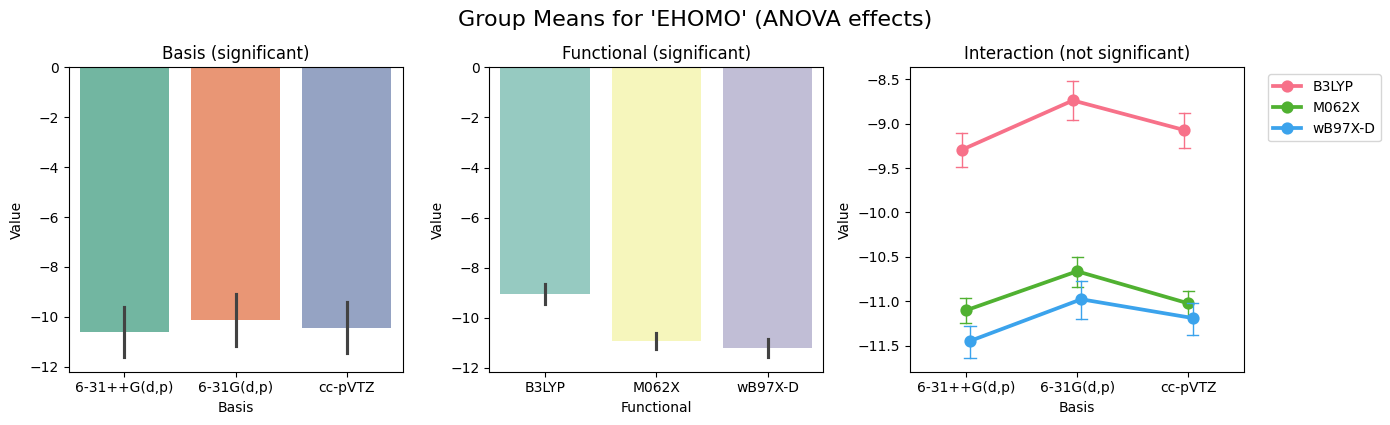
\includegraphics[width=\textwidth,height=\textheight,keepaspectratio]{Figures/anova_homo.png}
\caption{Group means for HOMO energy. Energy level seems to be changing across basis sets and growing with increasing functional complexity}
\label{anova_homo}
\end{figure}

\begin{figure}[H]
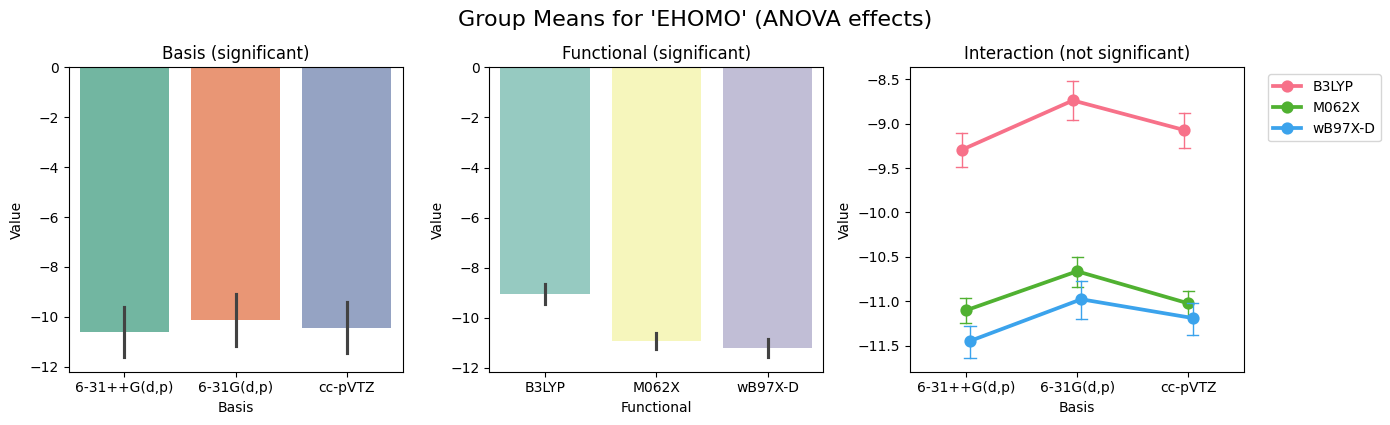
\includegraphics[width=\textwidth,height=\textheight,keepaspectratio]{Figures/anova_homo.png}
\caption{Group means for LUMO energy. Significant differences between different basis sets and functionals}
\label{anova_lumo}
\end{figure}

Both the basis set and functional independently influence the computed HOMO and LUMO energies. The lack of significant interaction indicates that the effect of one factor does not depend on the level of the other. EHOMO systematically deepens (more negative) when moving from B3LYP to M06-2X to ωB97X-D, and also shifts slightly downward with larger basis sets (Figures \ref{anova_homo} and \ref{anova_lumo}). Similarly, ELUMO energies shift upward or become more positive under functionals with more exact exchange and adjust modestly with basis size.


\subsection*{Descriptors with significant basis, functional, and interaction effects}

For Mu and Omega, all three effects were significant:

\begin{itemize}
    \item Mu: Basis (\(p = 1.45 \times 10^{-53}\)), Functional (\(p = 3.48 \times 10^{-31}\)), Interaction (\(p = 0.00506\))
    \item Omega: Basis (\(p = 2.96 \times 10^{-24}\)), Functional (\(p = 1.62 \times 10^{-42}\)), Interaction (\(p = 0.0155\))
\end{itemize}

\begin{figure}[H]
\centering
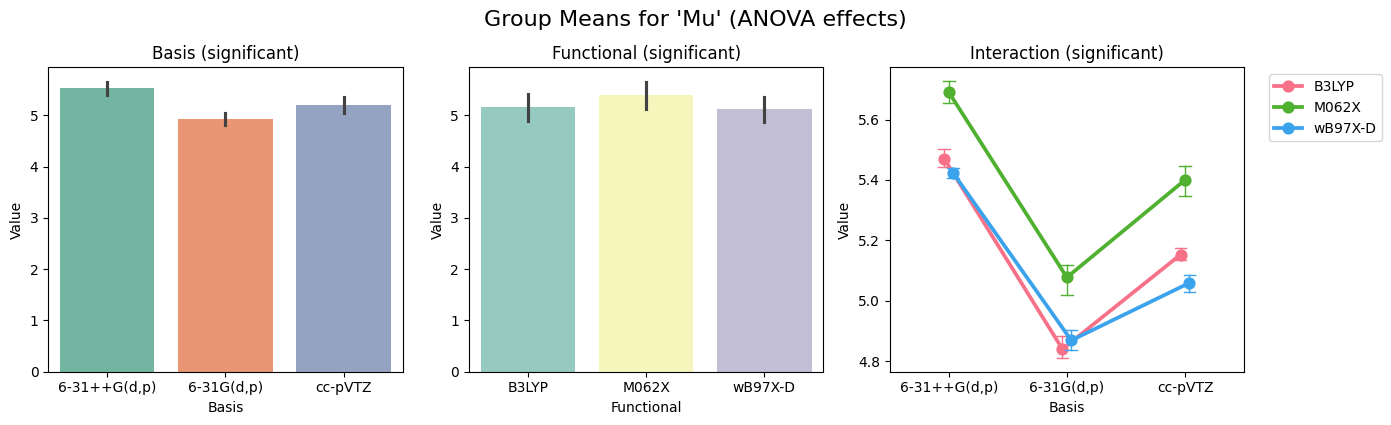
\includegraphics[width=\textwidth,height=\textheight,keepaspectratio]{Figures/anova_mu.png}
\caption{Group means for mu. Average value is smaller for 6-31G(d,p) basis set and larger for M062X functional}
\label{anova_mu}
\end{figure}

\begin{figure}[H]
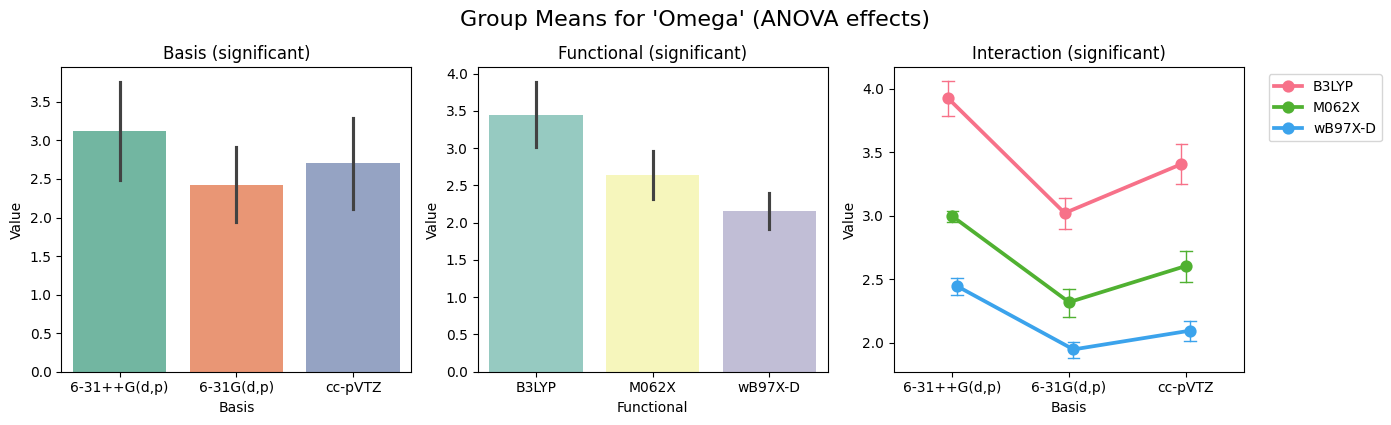
\includegraphics[width=\textwidth,height=\textheight,keepaspectratio]{Figures/anova_omega.png}
\caption{Group means for omega. The value is changing relative to the choice of basis set and dropping significantly with increasing functional complexity}
\label{anova_omega}
\end{figure}


 For chemical potential (Mu), mean values increase with larger basis sets but the magnitude of this increase differs by functional: e.g., M06-2X shows a larger rise from small to large basis than B3LYP or ωB97X-D (Figures \ref{anova_mu}). This interaction indicates that one cannot generalize a single basis effect across all functionals. For electrophilicity (Omega), values decrease going from B3LYP to M06-2X to ωB97X-D, and the basis-set enlargement moderates these shifts differently per functional Figure (\ref{anova_omega}). The visible trends underscore that both basis and functional choices jointly determine Mu and Omega, so a balanced mid-level combination (e.g., M06-2X/6-31++G(d,p)) may approximate higher-level results while controlling runtime.

Table~\ref{tab:anova-summary} summarizes the results of the two-way ANOVA performed for each descriptor and computational time, indicating which parameter(s) - basis set, functional, or their interaction - had a statistically significant effect.

\begin{table}[h!]
\centering
\caption{Summary of two-way ANOVA results for each descriptor. \textbf{Yes} = significant ($p < 0.05$), No = not significant.}
\begin{tabular}{lcccc}
\hline
\textbf{Descriptor} & \textbf{Basis} & \textbf{Functional} & \textbf{Interaction} & \textbf{Main Source of Variation} \\
\hline
LogP         & No  & No  & No  & None \\
TPSA         & No  & No  & No  & None \\
SASA         & No  & No  & No  & None \\
HF\_Energy   & No  & No  & No  & None \\
Dipole       & No  & No  & No  & None \\
Gap          & No  & \textbf{Yes} & No  & Functional \\
Hardness     & No  & \textbf{Yes} & No  & Functional \\
Softness     & No  & \textbf{Yes} & No  & Functional \\
EHOMO        & \textbf{Yes} & \textbf{Yes} & No  & Basis, Functional \\
ELUMO        & \textbf{Yes} & \textbf{Yes} & No  & Basis, Functional \\
Mu           & \textbf{Yes} & \textbf{Yes} & \textbf{Yes} & Basis, Functional, Interaction \\
Omega        & \textbf{Yes} & \textbf{Yes} & \textbf{Yes} & Basis, Functional, Interaction \\
Time         & \textbf{Yes} & No & No & Basis \\
\hline
\end{tabular}
\label{tab:anova-summary}
\end{table}


% --------------------------------------
% --------------------------------------
% --------------------------------------

\clearpage
\section{Machine learning results}
   

Using the descriptors (Sex, Species, LogP, SASA, Gap, HF energy) and dividing the nine PFAS compounds into a training set (6 compounds, as described above) and a test set (also described above), calculations were performed for nine basis sets with different functionals. Below are three tables corresponding to three machine learning methods – kNN, XGBoost, and Decision Tree (DT). The same descriptors were used in all calculations.

For the kNN algorithm (Table \ref{tab:my_table1}), the hyperparameter k was set to 3.
For XGBoost (Table \ref{tab:my_table2}), the parameters were: n estimators = 10, learning rate = 0.1, max depth = 3.
For the Decision Tree algorithm (Table \ref{tab:my_table3}), the parameters were: max depth = 3, min samples leaf = 10, min samples split = 3, random state = 42.

The results were compared in terms of performance using the calculated statistics: accuracy, precision, recall, and F1 score.


\begin{table}[H]
\centering
\caption{Results from all basis and functionals for kNN algorithm}
\begin{tabular}{|l |l |l |l |l |l |l |l |l|}\hline      
kNN& \multicolumn{2}{|c|}{Acuracy} & \multicolumn{2}{|c|}{Precision} & \multicolumn{2}{|c|}{Recall} & \multicolumn{2}{|c|}{F1} \\\hline
 & train & test & train & test & train & test & train & test \\\hline
6-31++G(d,p)-B3LYP & 0.947 & 0.818 & 0.953 & 0.709 & 0.947 & 0.818 & 0.947 & 0.75 \\\hline
6-31++G(d,p)-M062X & 0.947 & 0.818 & 0.953 & 0.709 & 0.947 & 0.818 & 0.947 & 0.75 \\\hline
6-31++G(d,p)-wB97X-D & 0.947 & 0.818 & 0.953 & 0.709 & 0.947 & 0.818 & 0.947 & 0.75 \\\hline
6-31G(d,p)-B3LYP & 0.947 & 0.818 & 0.953 & 0.709 & 0.947 & 0.818 & 0.947 & 0.75 \\\hline
6-31G(d,p)-M062X & 0.947 & 0.818 & 0.953 & 0.709 & 0.947 & 0.818 & 0.947 & 0.75 \\\hline
6-31G(d,p)-wB97X-D & 0.947 & 0.818 & 0.953 & 0.709 & 0.947 & 0.818 & 0.947 & 0.75 \\\hline
cc-pVTZ-B3LYP & 0.947 & 0.818 & 0.953 & 0.709 & 0.947 & 0.818 & 0.947 & 0.75 \\\hline
cc-pVTZ-M062X & 0.947 & 0.818 & 0.953 & 0.709 & 0.947 & 0.818 & 0.947 & 0.75 \\\hline
cc-pVTZ-wB97X-D & 0.947 & 0.818 & 0.953 & 0.709 & 0.947 & 0.818 & 0.947 & 0.75 \\ \hline

\end{tabular}
\label{tab:my_table1}
\end{table}


\begin{table}[H]
\centering
\caption{Results from all basis and functionals for XGBoost algorithm}
\begin{tabular}{|l |l |l |l |l |l |l |l |l|}\hline      
XGBoost& \multicolumn{2}{|c|}{Acuracy} & \multicolumn{2}{|c|}{Precision} & \multicolumn{2}{|c|}{Recall} & \multicolumn{2}{|c|}{F1} \\\hline
 & train & test & train & test & train & test & train & test \\\hline
6-31++G(d,p)-B3LYP & 0.929 & 0.727 & 0.942 & 0.609 & 0.929 & 0.727 & 0.929 & 0.660 \\\hline
6-31++G(d,p)-M062X & 0.929 & 0.727 & 0.942 & 0.609 & 0.929 & 0.727 & 0.929 & 0.660 \\\hline
6-31++G(d,p)-wB97X-D & 0.929 & 0.727 & 0.942 & 0.609 & 0.929 & 0.727 & 0.929 & 0.660 \\\hline
6-31G(d,p)-B3LYP & 0.929 & 0.727 & 0.942 & 0.609 & 0.929 & 0.727 & 0.929 & 0.660 \\\hline
6-31G(d,p)-M062X & 0.929 & 0.727 & 0.942 & 0.609 & 0.929 & 0.727 & 0.929 & 0.660 \\\hline
6-31G(d,p)-wB97X-D & 0.929 & 0.727 & 0.942 & 0.609 & 0.929 & 0.727 & 0.929 & 0.660 \\\hline
cc-pVTZ-B3LYP & 0.929 & 0.727 & 0.942 & 0.609 & 0.929 & 0.727 & 0.929 & 0.660 \\\hline
cc-pVTZ-M062X & 0.929 & 0.727 & 0.942 & 0.609 & 0.929 & 0.727 & 0.929 & 0.660 \\\hline
cc-pVTZ-wB97X-D & \textbf{0.894} & \textbf{0.909} & \textbf{0.899} & \textbf{0.927} & \textbf{0.894} & \textbf{0.909} & \textbf{0.895} & \textbf{0.905} \\ \hline

\end{tabular}
\label{tab:my_table2}
\end{table}



\begin{table}[H]
\centering
\caption{Results from all basis and functionals for DT algorithm}
\begin{tabular}{|l |l |l |l |l |l |l |l |l|}\hline      
DT & \multicolumn{2}{|c|}{Acuracy} & \multicolumn{2}{|c|}{Precision} & \multicolumn{2}{|c|}{Recall} & \multicolumn{2}{|c|}{F1} \\\hline
 & train & test & train & test & train & test & train & test \\\hline
6-31++G(d,p)-B3LYP & 0.807 & 0.727 & 0.848 & 0.609 & 0.807 & 0.727 & 0.809 & 0.660 \\\hline
6-31++G(d,p)-M062X & 0.807 & 0.727 & 0.848 & 0.609 & 0.807 & 0.727 & 0.809 & 0.660 \\\hline
6-31++G(d,p)-wB97X-D & 0.807 & 0.727 & 0.848 & 0.609 & 0.807 & 0.727 & 0.809 & 0.660 \\\hline
6-31G(d,p)-B3LYP & 0.807 & 0.727 & 0.848 & 0.609 & 0.807 & 0.727 & 0.809 & 0.660 \\\hline
6-31G(d,p)-M062X & 0.807 & 0.727 & 0.848 & 0.609 & 0.807 & 0.727 & 0.809 & 0.660 \\\hline
6-31G(d,p)-wB97X-D & 0.807 & 0.727 & 0.848 & 0.609 & 0.807 & 0.727 & 0.809 & 0.660 \\\hline
cc-pVTZ-B3LYP & 0.807 & 0.727 & 0.848 & 0.609 & 0.807 & 0.727 & 0.809 & 0.660 \\\hline
cc-pVTZ-M062X & 0.807 & 0.727 & 0.848 & 0.609 & 0.807 & 0.727 & 0.809 & 0.660 \\\hline
cc-pVTZ-wB97X-D & 0.736 & 0.727 & 0.772 & 0.609 & 0.736 & 0.727 & 0.737 & 0.660 \\ \hline

\end{tabular}

\label{tab:my_table3}
\end{table}

The results presented above apply to all tested databases and feature sets across three ma- chine learning algorithms — kNN, XGBoost, and DT. The cc-pVTZ-wB97X-D database in combination with the XGBoost algorithm achieved the best performance. These results are highlighted in bold in Table \ref{tab:my_table2}. For both the training and test sets, metrics such as accuracy, precision, recall, and F1 score are approximately 0.9, indicating very strong classification performance. Below is the confusion matrix  (Figure \ref{naj_conf_matrix}) for the aforementioned dataset. This represents the most accurate approach among those selected, although it is also the most time-consuming. In the training set, the XGBoost-based [Q]SPR model correctly classified:

\begin{itemize}
    \item 10 compounds in class 1
    \item 12 compounds in class 2
    \item 17 compounds in class 3
    \item 12 compounds in class 4
\end{itemize}
Six compounds were misclassified:
\begin{itemize}
    \item 1 compound from class 1 (perfluorooctanoic acid) was classified as class 3
    \item  3 compounds from class 2 (perfluorooctanoic acid and perfluorohexanesulfonic acid) were classified as class 3
    \item   2 compounds-rows from class 3 (perfluorobutanesulfonic acid for human male and female) were classified as class 2
\end{itemize}

This last type of misclassification is particularly concerning because class 3 corresponds to a half-life of less than 2 months, while class 2 corresponds to a half-life of less than one week. This means that the compound was mistakenly identified as less toxic than it actually is.

For the validation set, the algorithm correctly classified:
\begin{itemize}
    \item   4 compounds in class 1
    \item   4 compounds in class 2
    \item   8 compounds in class 3
    \item   4 compounds in class 4
\end{itemize}

Two compounds were misclassified:
\begin{itemize}
    \item from class 3 perfluorononanoic acid was classified as class 2
\end{itemize}

\begin{figure}[H]
    \centering
    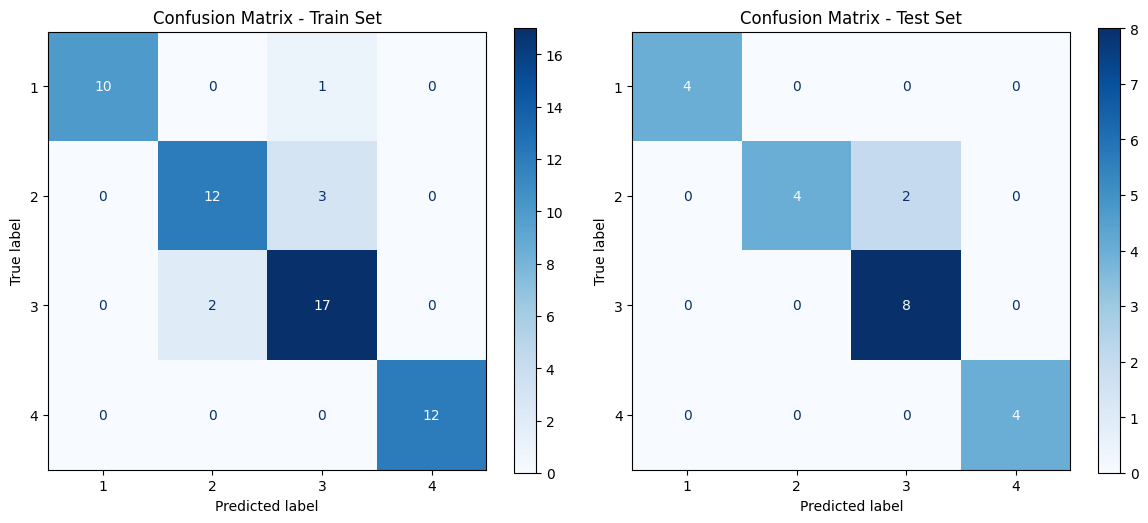
\includegraphics[width=\textwidth,height=\textheight,keepaspectratio]{Figures/naj_conf_matrix.png}
    \caption{Confusion matrix of the best-performing XGBoost-based [Q]SPR model for classifying PFAS into categories based on their half-life}
    \label{naj_conf_matrix}
\end{figure}



For better visualization of the data and results, the table below presents the data along with descriptors, the name of the compound, the class half lifetime, and the prediction from the selected model — XGB for $\omega$B97X-D/cc-pVTZ.


\begin{table}[H]
\caption{Dataset used during model development. Colored rows indicate incorrect prediction of half-life class.}
\resizebox{\textwidth}{!}{%
\begin{tabular}{|l|l|l|l|l|l|l|l|l|l|}
\hline
\textbf{Name} & \textbf{Species} & \textbf{Sex} & \textbf{LogP} & \textbf{SASA} & \textbf{Gap} & \textbf{HF\_Energy} & \textbf{T/V} & \textbf{Class half   lifetime} & \multicolumn{1}{c|}{\textbf{Predictions}} \\ \hline
GenX & Human & Male & 3.266 & 176.5496 & 12.0639 & -1553.3455 & T & 2 & 2 \\ \hline
GenX & Rat & Male & 3.266 & 176.5496 & 12.0639 & -1553.3455 & T & 2 & 2 \\ \hline
GenX & Monkey & Female & 3.266 & 176.5496 & 12.0639 & -1553.3455 & T & 2 & 2 \\ \hline
GenX & Rat & Male & 3.266 & 176.5496 & 12.0639 & -1553.3455 & T & 2 & 2 \\ \hline
GenX & Monkey & Male & 3.266 & 176.5496 & 12.0639 & -1553.3455 & T & 2 & 2 \\ \hline
GenX & Rat & Female & 3.266 & 176.5496 & 12.0639 & -1553.3455 & T & 2 & 2 \\ \hline
GenX & Human & Female & 3.266 & 176.5496 & 12.0639 & -1553.3455 & T & 2 & 2 \\ \hline
GenX & Rat & Female & 3.266 & 176.5496 & 12.0639 & -1553.3455 & T & 2 & 2 \\ \hline
GenX & Mouse & Female & 3.266 & 176.5496 & 12.0639 & -1553.3455 & T & 2 & 2 \\ \hline
GenX & Mouse & Male & 3.266 & 176.5496 & 12.0639 & -1553.3455 & T & 2 & 2 \\ \hline
Perfluoroheptanoic   acid & Human & Male & 5.0318 & 193.5779 & 11.7148 & -1715.9077 & T & 4 & 4 \\ \hline
Perfluoroheptanoic   acid & Rat & Male & 5.0318 & 193.5779 & 11.7148 & -1715.9077 & T & 1 & 1 \\ \hline
Perfluoroheptanoic   acid & Rat & Female & 5.0318 & 193.5779 & 11.7148 & -1715.9077 & T & 1 & 1 \\ \hline
Perfluoroheptanoic   acid & Rat & Female & 5.0318 & 193.5779 & 11.7148 & -1715.9077 & T & 1 & 1 \\ \hline
Perfluoroheptanoic   acid & Human & Female & 5.0318 & 193.5779 & 11.7148 & -1715.9077 & T & 4 & 4 \\ \hline
Perfluoroheptanoic   acid & Rat & Male & 5.0318 & 193.5779 & 11.7148 & -1715.9077 & T & 1 & 1 \\ \hline
Perfluorooctanoic   acid & Monkey & Male & 5.9729 & 219.0702 & 11.7338 & -1953.7174 & T & 3 & 3 \\ \hline
Perfluorooctanoic   acid & Rat & Male & 5.9729 & 219.0702 & 11.7338 & -1953.7174 & T & 3 & 3 \\ \hline
Perfluorooctanoic   acid & Human & Male & 5.9729 & 219.0702 & 11.7338 & -1953.7174 & T & 4 & 4 \\ \hline
Perfluorooctanoic   acid & Mouse & Male & 5.9729 & 219.0702 & 11.7338 & -1953.7174 & T & 3 & 3 \\ \hline
\rowcolor[HTML]{DAE9F8} 
Perfluorooctanoic   acid & Rat & Female & 5.9729 & 219.0702 & 11.7338 & -1953.7174 & T & 2 & 3 \\ \hline
Perfluorooctanoic   acid & Rat & Male & 5.9729 & 219.0702 & 11.7338 & -1953.7174 & T & 3 & 3 \\ \hline
Perfluorooctanoic   acid & Monkey & Male & 5.9729 & 219.0702 & 11.7338 & -1953.7174 & T & 3 & 3 \\ \hline
Perfluorooctanoic   acid & Mouse & Female & 5.9729 & 219.0702 & 11.7338 & -1953.7174 & T & 3 & 3 \\ \hline
\rowcolor[HTML]{DAE9F8} 
Perfluorooctanoic   acid & Rat & Female & 5.9729 & 219.0702 & 11.7338 & -1953.7174 & T & 1 & 3 \\ \hline
Perfluorooctanoic   acid & Human & Female & 5.9729 & 219.0702 & 11.7338 & -1953.7174 & T & 4 & 4 \\ \hline
Perfluorooctanoic   acid & Monkey & Female & 5.9729 & 219.0702 & 11.7338 & -1953.7174 & T & 3 & 3 \\ \hline
Perfluorooctanesulfonic   acid & Mouse & Female & 5.566 & 255.4005 & 12.8136 & -2626.7966 & T & 3 & 3 \\ \hline
Perfluorooctanesulfonic   acid & Human & Female & 5.566 & 255.4005 & 12.8136 & -2626.7966 & T & 4 & 4 \\ \hline
Perfluorooctanesulfonic   acid & Monkey & Female & 5.566 & 255.4005 & 12.8136 & -2626.7966 & T & 4 & 4 \\ \hline
Perfluorooctanesulfonic   acid & Human & Male & 5.566 & 255.4005 & 12.8136 & -2626.7966 & T & 4 & 4 \\ \hline
Perfluorooctanesulfonic   acid & Rat & Female & 5.566 & 255.4005 & 12.8136 & -2626.7966 & T & 3 & 3 \\ \hline
Perfluorooctanesulfonic   acid & Mouse & Male & 5.566 & 255.4005 & 12.8136 & -2626.7966 & T & 3 & 3 \\ \hline
Perfluorooctanesulfonic   acid & Rat & Male & 5.566 & 255.4005 & 12.8136 & -2626.7966 & T & 3 & 3 \\ \hline
Perfluorooctanesulfonic   acid & Monkey & Male & 5.566 & 255.4005 & 12.8136 & -2626.7966 & T & 4 & 4 \\ \hline
Perfluorooctanesulfonic   acid & Rat & Male & 5.566 & 255.4005 & 12.8136 & -2626.7966 & T & 3 & 3 \\ \hline
Perfluorooctanesulfonic   acid & Rat & Female & 5.566 & 255.4005 & 12.8136 & -2626.7966 & T & 3 & 3 \\ \hline
Perfluorobutanesulfonic   acid & Rat & Female & 1.8016 & 153.4312 & 13.0892 & -1675.5 & T & 1 & 1 \\ \hline
Perfluorobutanesulfonic   acid & Monkey & Male & 1.8016 & 153.4312 & 13.0892 & -1675.5 & T & 2 & 2 \\ \hline
Perfluorobutanesulfonic   acid & Mouse & Female & 1.8016 & 153.4312 & 13.0892 & -1675.5 & T & 1 & 1 \\ \hline
Perfluorobutanesulfonic   acid & Mouse & Male & 1.8016 & 153.4312 & 13.0892 & -1675.5 & T & 1 & 1 \\ \hline
\rowcolor[HTML]{DAE9F8} 
Perfluorobutanesulfonic   acid & Human & Male & 1.8016 & 153.4312 & 13.0892 & -1675.5 & T & 3 & 2 \\ \hline
Perfluorobutanesulfonic   acid & Rat & Male & 1.8016 & 153.4312 & 13.0892 & -1675.5 & T & 1 & 1 \\ \hline
Perfluorobutanesulfonic   acid & Monkey & Female & 1.8016 & 153.4312 & 13.0892 & -1675.5 & T & 2 & 2 \\ \hline
Perfluorobutanesulfonic   acid & Rat & Male & 1.8016 & 153.4312 & 13.0892 & -1675.5 & T & 1 & 1 \\ \hline
\rowcolor[HTML]{DAE9F8} 
Perfluorobutanesulfonic   acid & Human & Female & 1.8016 & 153.4312 & 13.0892 & -1675.5 & T & 3 & 2 \\ \hline
Perfluorobutanesulfonic   acid & Rat & Female & 1.8016 & 153.4312 & 13.0892 & -1675.5 & T & 1 & 1 \\ \hline
Perfluorohexanesulfonic   acid & Mouse & Female & 3.6838 & 204.4159 & 12.8838 & -2151.1801 & T & 3 & 3 \\ \hline
Perfluorohexanesulfonic   acid & Rat & Male & 3.6838 & 204.4159 & 12.8838 & -2151.1801 & T & 3 & 3 \\ \hline
Perfluorohexanesulfonic   acid & Human & Male & 3.6838 & 204.4159 & 12.8838 & -2151.1801 & T & 4 & 4 \\ \hline
Perfluorohexanesulfonic   acid & Human & Female & 3.6838 & 204.4159 & 12.8838 & -2151.1801 & T & 4 & 4 \\ \hline
Perfluorohexanesulfonic   acid & Monkey & Male & 3.6838 & 204.4159 & 12.8838 & -2151.1801 & T & 4 & 4 \\ \hline
Perfluorohexanesulfonic   acid & Rat & Male & 3.6838 & 204.4159 & 12.8838 & -2151.1801 & T & 3 & 3 \\ \hline
Perfluorohexanesulfonic   acid & Mouse & Male & 3.6838 & 204.4159 & 12.8838 & -2151.1801 & T & 3 & 3 \\ \hline
\rowcolor[HTML]{DAE9F8} 
Perfluorohexanesulfonic   acid & Rat & Female & 3.6838 & 204.4159 & 12.8838 & -2151.1801 & T & 2 & 3 \\ \hline
\rowcolor[HTML]{DAE9F8} 
Perfluorohexanesulfonic   acid & Rat & Female & 3.6838 & 204.4159 & 12.8838 & -2151.1801 & T & 2 & 3 \\ \hline
Perfluorohexanesulfonic   acid & Monkey & Female & 3.6838 & 204.4159 & 12.8838 & -2151.1801 & T & 4 & 4 \\ \hline

\end{tabular}%
}
\end{table}


\begin{table}[H]
\resizebox{\textwidth}{!}{%
\begin{tabular}{|l|l|l|l|l|l|l|l|l|l|}
\hline
\textbf{Name} & \textbf{Species} & \textbf{Sex} & \textbf{LogP} & \textbf{SASA} & \textbf{Gap} & \textbf{HF\_Energy} & \textbf{T/V} & \textbf{Class half   lifetime} & \multicolumn{1}{c|}{\textbf{Predictions}} \\ \hline
Perfluorononanoic   acid & Rat & Male & 6.914 & 244.5625 & 11.7295 & -2191.5274 & V & 3 & 3 \\ \hline
Perfluorononanoic   acid & Human & Male & 6.914 & 244.5625 & 11.7295 & -2191.5274 & V & 4 & 4 \\ \hline
Perfluorononanoic   acid & Human & Female & 6.914 & 244.5625 & 11.7295 & -2191.5274 & V & 4 & 4 \\ \hline
Perfluorononanoic   acid & Rat & Male & 6.914 & 244.5625 & 11.7295 & -2191.5274 & V & 3 & 3 \\ \hline
Perfluorononanoic   acid & Mouse & Female & 6.914 & 244.5625 & 11.7295 & -2191.5274 & V & 3 & 3 \\ \hline
\rowcolor[HTML]{DAE9F8} 
Perfluorononanoic   acid & Rat & Female & 6.914 & 244.5625 & 11.7295 & -2191.5274 & V & 2 & 3 \\ \hline
\rowcolor[HTML]{DAE9F8} 
Perfluorononanoic   acid & Rat & Female & 6.914 & 244.5625 & 11.7295 & -2191.5274 & V & 2 & 3 \\ \hline
Perfluorononanoic   acid & Mouse & Male & 6.914 & 244.5625 & 11.7295 & -2191.5274 & V & 3 & 3 \\ \hline
Perfluorobutanoic   acid & Human & Female & 2.2085 & 117.1009 & 11.6995 & -1002.4773 & V & 2 & 2 \\ \hline
Perfluorobutanoic   acid & Monkey & Male & 2.2085 & 117.1009 & 11.6995 & -1002.4773 & V & 2 & 2 \\ \hline
Perfluorobutanoic   acid & Monkey & Female & 2.2085 & 117.1009 & 11.6995 & -1002.4773 & V & 2 & 2 \\ \hline
Perfluorobutanoic   acid & Human & Male & 2.2085 & 117.1009 & 11.6995 & -1002.4773 & V & 2 & 2 \\ \hline
Perfluorobutanoic   acid & Rat & Male & 2.2085 & 117.1009 & 11.6995 & -1002.4773 & V & 1 & 1 \\ \hline
Perfluorobutanoic   acid & Mouse & Male & 2.2085 & 117.1009 & 11.6995 & -1002.4773 & V & 1 & 1 \\ \hline
Perfluorobutanoic   acid & Mouse & Female & 2.2085 & 117.1009 & 11.6995 & -1002.4773 & V & 1 & 1 \\ \hline
Perfluorobutanoic   acid & Rat & Female & 2.2085 & 117.1009 & 11.6995 & -1002.4773 & V & 1 & 1 \\ \hline
Perfluorodecanoic   acid & Human & Male & 7.8551 & 270.0549 & 11.7292 & -2429.3374 & V & 4 & 4 \\ \hline
Perfluorodecanoic   acid & Rat & Female & 7.8551 & 270.0549 & 11.7292 & -2429.3374 & V & 3 & 3 \\ \hline
Perfluorodecanoic   acid & Rat & Male & 7.8551 & 270.0549 & 11.7292 & -2429.3374 & V & 3 & 3 \\ \hline
Perfluorodecanoic   acid & Rat & Male & 7.8551 & 270.0549 & 11.7292 & -2429.3374 & V & 3 & 3 \\ \hline
Perfluorodecanoic   acid & Rat & Female & 7.8551 & 270.0549 & 11.7292 & -2429.3374 & V & 3 & 3 \\ \hline
Perfluorodecanoic   acid & Human & Female & 7.8551 & 270.0549 & 11.7292 & -2429.3374 & V & 4 & 4 \\ \hline
\end{tabular}%
}
\end{table}

Of particular note is the fact that the average computation time required to perform geometry optimization and calculate descriptors for a single compound was 39 hours, as shown in (Figure \ref{times}). Due to the significant time and computational costs involved, as well as the fact that the best-performing descriptor calculation method described above did not substantially improve classification results compared to other considered methods, the question of balancing accuracy with computational efficiency arises. It is important to remember that \textit{in silico} models, including the [Q]SPR model developed in this master’s thesis, are approximations of experimental results.
     

\begin{figure}[H]
    \centering
    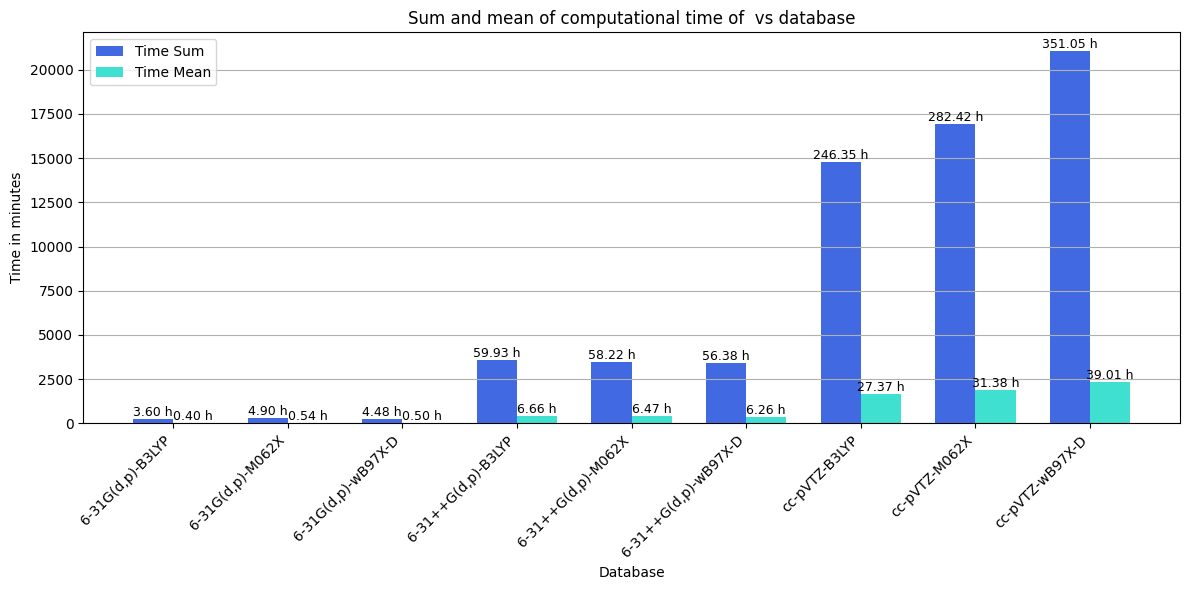
\includegraphics[width=\textwidth,height=\textheight,keepaspectratio]{Figures/times_sum_mean.png}
    \caption{Bar plot, of the sum and mean of the computational time for the considered DFT methods (combining various functionals with different basis sets).}
    \label{times}
\end{figure}

It can be seen that for many basis sets and functionals, the results are very similar. For example, in the case of the kNN algorithm, the evaluation statistics are the same for several combinations.
When comparing a model that has lower performance based on the calculated statistics but much shorter computation time, this observation becomes even clearer. For example, for the 6-31++G(d,p) basis set with the M06-2X functional, the confusion matrix for the XGBoost algorithm is shown in the figure \ref{conf_M062}.


From the results table above, it can be observed that the model is slightly overfitted, as the accuracy for the training data is 0.92, while for the test data it drops to 0.72.
The confusion matrix shows good prediction performance for the training set, with only 3 compounds misclassified.
However, for the test set, as before, 2 compounds were incorrectly assigned to class 3 instead of class 2. Additionally, in this case, no compound was correctly classified into class 1.

\begin{figure}[H]
    \centering
    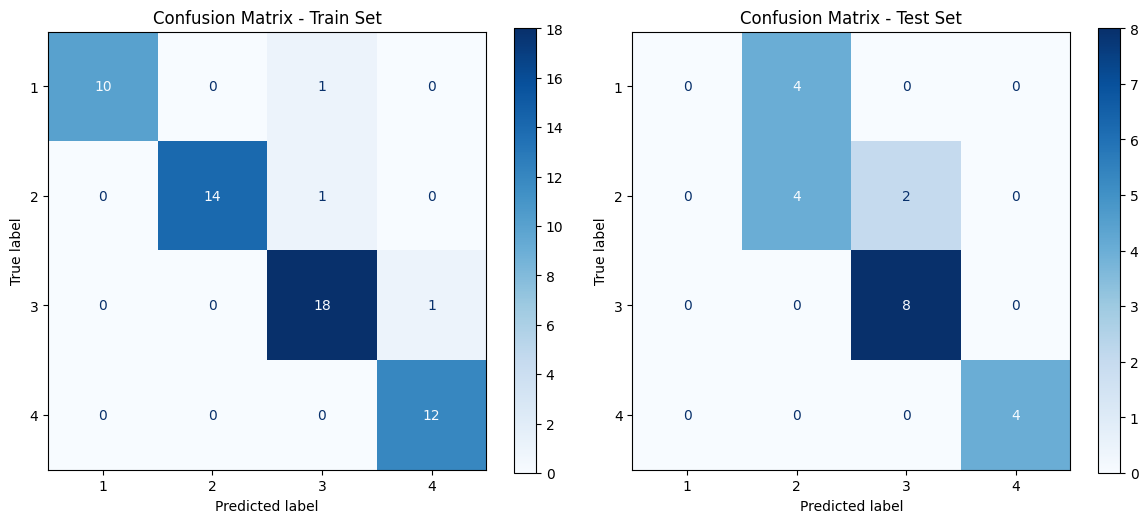
\includegraphics[width=\textwidth,height=\textheight,keepaspectratio]{Figures/conf_matrix_m062.png}
    \caption{Confusion matrix for XGBoost classifier trained and tested for M06-2X/6-31++G(d,p)}
    \label{conf_M062}
\end{figure}


The XGBoost model's feature importance analysis, based on gain values, highlights the HOMO-LUMO gap as the most influential feature, contributing 27\% to the model's predictive power. This is followed by SASA at 23\%, and HF energy at 17\%, indicating the dominant role of electronic and structural molecular properties. Species identity and logP also play substantial roles, contributing 16\% and 15\%, respectively. Notably, Sex shows minimal influence at only 3\%, suggesting that the molecular features are the primary drivers of the model's performance, while demographic factors like sex have limited predictive value in this context \ref{fig:feature_importance}.

\begin{figure}[H]
    \centering
    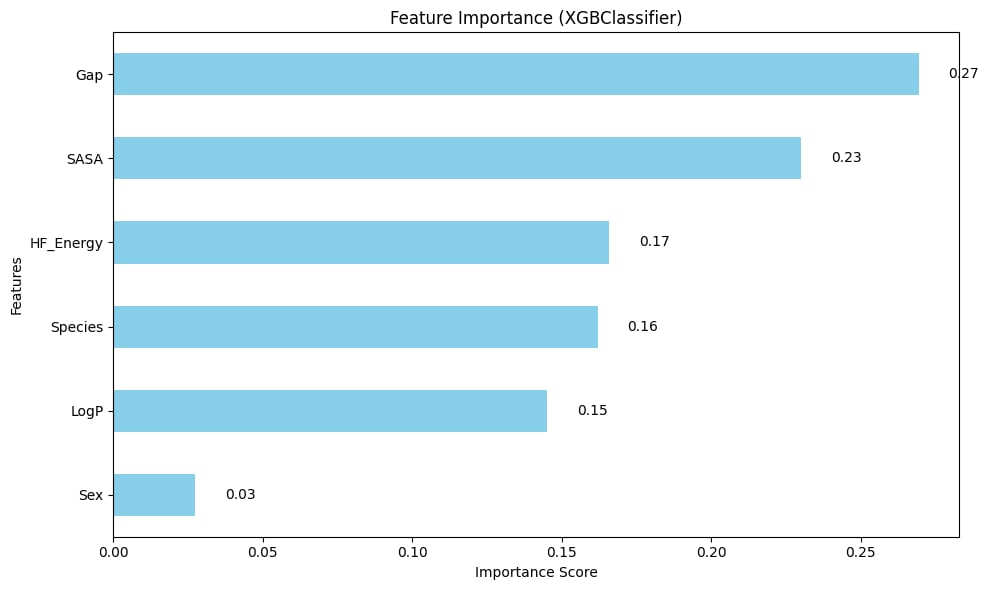
\includegraphics[width=\textwidth,height=\textheight,keepaspectratio]{Figures/feataure_imporatnce.jpg}
    \caption{Feature importance plot for XGB algorithm for the most accurate model.}
    \label{fig:feature_importance}
\end{figure}
% #wykres dodamy w wynikach

% -------------------------------------------
% -------------------------------------------
% -------------------------------------------
% -------------------------------------------
% -------------------------------------------

\chapter{Discussion}

In this section, we interpret the findings from both the DFT-derived descriptor analysis and the machine learning experiments. Specifically, we examine how methodological choices, particularly the basis set, functional, influence descriptor values and their reliability in classifying PFAS persistence. We also explore the trade-offs between computational cost and descriptor accuracy. Next, we evaluate the performance of these descriptors in PFAS half-life category classification models. Finally, we compare different ML algorithms and descriptor sets and reflect on the earlier outlined research hypotheses and objectives.

\subsection{DFT-derived descriptors: influence of functional and basis set}

A central aim of this master’s thesis was to understand how the choice of exchange–correlation functional and basis set affect the computed molecular descriptors that may correlate with PFAS persistence (Objectives 1 and 2). The results of two-way ANOVA revealed distinct patterns. Descriptors such as LogP, TPSA, SASA, HF energy, and dipole moment were largely unaffected by the basis set or functional choice (all \(p>0.05\)). These results suggest that a modest level of theor (e.g., \texttt{B3LYP}/\texttt{6-31G(d,p)}) ) is sufficient to obtain stable values for these properties. From a practical standpoint, these descriptors can be efficiently computed with minimal sensitivity to methodological variation, enabling the allocation of computational resources toward more sensitive quantities.

In contrast, the energies of frontier orbitals (i.e., EHOMO and ELUMO) showed significant dependence on both the basis set and the functional. This suggests that predicted orbital levels and derived descriptors, such as the HOMO-LUMO gap, and chemical hardness, are sensitive to the level of theory. Specifically, the energies of the HOMO and LUMO energies became more negative with increasing basis set size and with functionals containing a higher proportion of exact exchange. Since the HOMO–LUMO gap is fundamental to secondary descriptors such as chemical hardness (\(\eta\)), chemical softness, chemical potential (\(\mu\)), and electrophilicity (\(\omega\)), these properties also varied significantly with methodological choices. Notably, the HOMO–LUMO gap, chemical hardness and chemical softness were significantly affected by the functional alone, while \(\mu\) and \(\omega\) were influenced by the basis set, functional, and their interaction. These results suggest that, although HOMO–LUMO gap-related descriptors are primarily sensitive to the exchange–correlation treatment, the basis set and functional play critical roles in determining chemical potential and electrophilicity. 

From a chemical perspective, descriptors related to frontier orbitals are key to understanding PFAS stability. Larger HOMO–LUMO gaps and higher chemical hardness are generally associated with greater resistance to oxidative or reductive degradation and therefore longer half-lives. However, their sensitivity to the computational method implies that selecting an appropriate level of theory is essential to balancing accuracy and computational feasibility. For example, \texttt{B3LYP}/\texttt{6-31G(d,p)} can capture qualitative trends, such as the relative ordering among PFAS classes, but it tends to underestimate HOMO–LUMO gap values compared to higher-level methods, such as (e.g., \texttt{\(\omega\)B97X-D}/\texttt{cc-pVTZ}). While the latter provides more robust quantitative results, it comes at a significantly higher computational cost. 

The significant interaction effects observed for \(\mu\) and \(\omega\) imply that the impact of the functional on these descriptors depends on the basis set size and \textit{vice versa}. In practice, using a mid-level basis set (e.g., \texttt{6-31++G(d,p)}) with a balanced functional (e.g., \texttt{M06-2X}) yields descriptor values that closely approximate those of high-level methods while maintaining manageable runtimes. When comparing HOMO–LUMO gaps computed at \texttt{M06‑2X/6‑31++G(d,p)} to those obtained at the higher-level \texttt{M06‑2X/cc‑pVTZ} level, deviations of approximately 0.2–0.3 eV are observed for perfluoroalkyl carboxylates, while sulfonates and bulkier PFAS compounds exhibit larger deviations ranging from $\sim$0.5 to 0.9 eV. Notably, despite these differences, no degradation in predictive performance was observed in machine learning models trained on either descriptor set, indicating the adequacy of the more affordable \texttt{M06‑2X/6‑31++G(d,p)} method for model construction in this context. Thus, for large-scale descriptor generation (Objective 3), this level of theory appears to offer a practical compromise—capturing essential electronic structure features relevant to PFAS persistence while operating at approximately one-tenth the computational cost of \texttt{cc‑pVTZ}.

Overall, these findings support research hypotheses H2 and H3 that descriptor quality and model performance vary depending on the chosen DFT method, and that more expensive methods do not necessarily offer the best trade-off. The invariance of certain descriptors suggests that they can be reliably computed at low cost, while more method-sensitive descriptors require careful methodological selection.

\subsection{Descriptor trends and PFAS persistence insights}

Beyond methodological sensitivity, the absolute and relative values of molecular descriptors reveal the distinct chemical characteristics of PFAS classes:

\paragraph{HOMO–LUMO gap, chemical hardness, chemical softness.} 
Sulfonates and bulky compounds, such as F53B, consistently exhibit larger HOMO–LUMO gaps and greater chemical hardness than carboxylates with similar chain lengths. This aligns with their known environmental and biological persistence \cite{F53B_worse} \cite{F53B_worse_2}. GenX occupies an intermediate position, reflecting its hybrid structural nature. This trend highlights the importance of frontier orbital-derived descriptors in modeling persistence; greater chemical hardness correlates with slower degradation pathways in both the environment and \textit{in vivo}. Since the HOMO–LUMO gap and chemical hardness are sensitive to computational methods, it is crucial to maintain consistent calculation settings when comparing different compounds.

\paragraph{Chemical potential and electrophilicity.} 
Sulfonates and F53B tend to have slightly more negative chemical potentials and lower electrophilicity indices than simpler carboxylates. This indicates a reduced tendency to participate in electron-accepting reactions. Though the differences in \(\mu\) and \(\omega\) are modest, they corroborate the observed chemical hardness trends and further differentiate PFAS compounds by their expected reactivity. Given their sensitivity to basis sets and functionals, mid-level DFT settings are recommended for reliable comparative studies

\paragraph{Dipole moment and polarity descriptors.} 
Dipole moments exhibit moderate dependence on the computational method, yet they maintain the relative order among PFAS classes. Sulfonates and F53B are more polar than carboxylates \cite{pfas_polarity_soil} \cite{pfas_protein_binding_dipole}. This indicates stronger interactions with aqueous environment and proteins, and contributes to longer biological residence times. TPSA and SASA values remain nearly constant across computational settings, confirming that these size- and topology-based descriptors can be reliably obtained from quick geometry optimizations.

\paragraph{LogP and HF energy.} 
LogP and total HF energy demonstrate negligible sensitivity to DFT settings in this master’s project. LogP remains a key indicator of bioaccumulation potential, while HF energy primarily confirms stable geometry convergence. Their robustness across methods allows for their inclusion in modeling without significant computational cost, particularly in the case of LogP, which can be calculated without the 3D structure optimization.

Taken together, these descriptor trends support the research hypothesis that PFAS persistence arises from a combination of electronic stability (i.e., a large HOMO–LUMO gap and high chemical hardness) and physicochemical features (i.e., high lipophilicity and polarity, which enable uptake and binding). These findings justify including both physichocemial descriptors (TPSA, LogP, and SASA) and DFT-derived electronic descriptors in classification models (supporting hypothesis - H1).

\subsection{Computational trade-offs}

Calculation time scaled steeply with basis set size and functional complexity, especially for larger PFAS like F53B. While high-level settings (e.g., \texttt{\(\omega\)B97X-D}/\texttt{cc-pVTZ}) should yield the most accurate electronic descriptors, the runtime (exceeding tens of hours per compound) limits throughput. Conversely, low-level combinations (e.g., \texttt{B3LYP}/\texttt{6-31G(d,p)}) deliver rapid geometry optimizations and stable topological descriptors but underperform on gap accuracy. Mid-level combinations (e.g., \texttt{M06-2X}/\texttt{6-31++G(d,p)}) emerged as a compromise, producing electronic descriptors close to high-level references at a fraction of the cost, which is crucial for large PFAS libraries. These observations align with Hypothesis H3 and guide recommendations for future large-scale PFAS descriptor generation workflows.

\subsection{Machine learning model performance}

This section examines how descriptors contribute to the classification of PFAS half-life categories (Objectives 4 and 5, and Hypotheses H1 and H4). Three algorithms — k-nearest neighbors, extreme gradient boosting, and decision tree — were evaluated using descriptor sets derived from each DFT method and from a physicochemical-only baseline.

\paragraph{Overall accuracy and best-performing combinations.} The highest classification metrics (accuracy, precision, recall, F1 $\sim$0.9 on test data) were achieved using descriptors from \texttt{\(\omega\)B97X-D}/\texttt{cc-pVTZ} with XGB. This confirms that including high-fidelity electronic descriptors can improve model accuracy, supporting H1. However, the marginal gain over mid-level settings may be modest relative to computational cost. For example, mid-level descriptors (\texttt{M06-2X}/\texttt{6-31++G(d,p)}) combined with 1D and 2D features may yield comparable performance.

\clearpage
\paragraph{Algorithm choice.} 
XGBoost consistently outperformed kNN and DT on the test data. This suggests that ensemble methods more effectively capture complex, nonlinear relationships among descriptors and model’s response. While ensemble methods such as XGBoost are powerful, they may also carry an increased risk of overfitting, particularly in small datasets. Decision trees showed limited generalizability, likely due to overfitting on the relatively small PFAS dataset, while kNN yielded stable but less accurate results compared to XGBoost. These findings support H4 that algorithm selection significantly impacts model performance. While simpler models may be more interpretable, they often sacrifice predictive accuracy.

\paragraph{Role of DFT descriptors versus 1D and 2D-only models.}
Models based solely on 1D and 2D descriptors achieved similar levels of performance when enhanced with additional features. However, the integration of electronic-structure information offered clear benefits. Feature importance analysis revealed that the HOMO-LUMO gap was among the top contributors to distinguishing between half-life categories. This validates the utility of DFT-derived descriptors (supporting first research hypothesis, H1). However, when mid-level descriptors were employed, the performance gap narrowed. This suggests that carefully selected DFT settings can improve model performance without incurring excessive computational costs (Figure \ref{fig:feature_importance}).

\paragraph{Misclassification analysis and risk implications.} 
The confusion matrix for the top- performing [Q]SPR model revealed misclassifications, particularly between categories with adjacent half-life ranges. Misclassifying a compound with a short half-life as longer-lived (or vice versa) has important implications for risk assessment. The most critical errors occurred when compounds with true half-life of less than two months were misclassified as having half-lives under one week. This could lead to an underestimation of environmental persistence. These findings underscore the need for cautious interpretation of model outputs and suggest that combining model’s predictions with expert judgment or testing is essential.

\paragraph{Computational efficiency and scalability.}
Although the highest accuracy was achieved with the most computationally intensive descriptor set, the performance differences relative to mid-level DFT settings were not substantial. Considering the average computation time per compound (e.g., 39 hours for high-level methods), using mid-level DFT descriptors (6-31++G(d,p)-M062X) or selectively incorporating electronic descriptors may be more scalable for large PFAS libraries. A tiered strategy, such as pre-screening with cheminformatics models followed by targeted DFT calculations for borderline cases, could optimize this process. This finding supports hypothesis H3: an optimal balance between accuracy and computational efficiency can be achieved through strategic model design.

\subsection{Limitations and future directions}

Several limitations of this master’s project should be acknowledged. First, the dataset size is relatively small at only ten molecules, so classification into half-life categories may lack representativeness. To improve model generalizability, it is necessary to expand the dataset to include a larger and more diverse set of PFAS compounds. Second, DFT-derived descriptors do not account for the complexity of biological environments, such as interactions within living organisms. They also cannot incorporate species- or gender-specific differences. Third, ML models depend on available experimental half-life data, which may vary in quality and consistency. Enhanced data curation and harmonization are therefore essential. Fourth, although mid-level DFT methods provided a practical balance between accuracy and computational cost, benchmarking against higher-level correlated methods or experimental data would strengthen confidence in the reliability of the descriptors.

Future research should focus on the following: (i) extending the generation of descriptors to a broader PFAS library; (ii) exploring additional electronic descriptors (e.g. excited-state properties and redox potentials) where applicable; (iii) evaluating deep learning architectures for classification tasks; and (iv) developing adaptive workflows that dynamically allocate computational resources based on initial chemoinformatics screening.
 
% Chapter 6

\chapter{Conclusion}

\label{Chapter6}

%---------------------------------------------------------------------------------------- 
\newcommand{\keyword}[1]{\textbf{#1}}
\newcommand{\tabhead}[1]{\textbf{#1}}
\newcommand{\code}[1]{\texttt{#1}}
\newcommand{\file}[1]{\texttt{\bfseries#1}}
\newcommand{\option}[1]{\texttt{\itshape#1}}
\renewcommand{\figurename}{Figure.}
\renewcommand{\tablename}{Table.}

%----------------------------------------------------------------------------------------
Completing all the objectives of this master's thesis verified the research hypotheses and led to the following conclusions:

\begin{enumerate}
  \item DFT-derived descriptors (i.e., HOMO–LUMO gap, solvent accessible surface area, Hartree–Fock energy) improve PFAS half-life classification when integrated with biological descriptors (i.e., Sex, Species) and physicochemical properties (i.e., logP);
  
  \item The choice of computational method influences descriptor sensitivity and overall model performance;
  
  \item A balanced, mid-level DFT approach (e.g., M06-2X/6-31++G(d,p)) often provides the optimal trade-off between accuracy and efficiency;
  
  \item Ensemble learning (e.g., XGBoost) effectively utilizes the descriptor set; however, considerations of interpretability and computational cost remain important.
\end{enumerate}

These findings offer a practical workflow for classifying PFAS persistence, advancing predictive toxicokinetic modeling, and supporting safer chemical design and informed regulatory decision-making.



%----------------------------------------------------------------------------------------
%	THESIS CONTENT - FIGURES AND TABLES
%----------------------------------------------------------------------------------------
\listoffigures
\listoftables

%----------------------------------------------------------------------------------------
%	BIBLIOGRAPHY
%----------------------------------------------------------------------------------------
\renewcommand\bibname{Bibliography}
\printbibliography[]

%----------------------------------------------------------------------------------------
%	DECLARATION PAGE
%----------------------------------------------------------------------------------------

\begin{declaration}
\addchaptertocentry{\authorshipname}
\begin{figure}[H]

\includegraphics[width=1\textwidth, center]{declaration_JR.png}
\end{figure}

\vspace{2cm}
 \begin{figure}[H]

\includegraphics[width=1\textwidth, center]{declaration_JN.png}
\end{figure}

\vspace{2cm}
 \begin{figure}[H]

\includegraphics[width=1\textwidth, center]{consent.png}
\end{figure}

\end{declaration}
\end{document}
